% =====================================================================
% MIKU SCI 小论文 — 中文稿
% 自包含可编译骨架，编译命令： latexmk -xelatex v4.tex
% =====================================================================
\documentclass[a4paper,11pt]{ctexart}

\usepackage{amsmath,amssymb,amsthm}
\usepackage{booktabs}
\usepackage{graphicx}
\usepackage{enumitem}
\usepackage{geometry}
\usepackage[ruled,vlined,linesnumbered]{algorithm2e}
\usepackage{tikz}
\usetikzlibrary{shapes.geometric, arrows.meta, positioning, fit, backgrounds, calc, patterns, decorations.pathreplacing}
\usepackage{caption}
\usepackage{subcaption}
\usepackage{float}
\usepackage{adjustbox}
\usepackage{pgfplots}
\pgfplotsset{compat=1.18}
\usepgfplotslibrary{fillbetween}
\pgfplotsset{table/search path={../../图片, ../../图片/data}}
\providecommand{\datapath}{../../图片/data/01_crossing_ped/}
% 概念图内部引用的示例参数宏，给出缺省值以保证自包含编译
\providecommand{\PedExampleS}{10.0}
\providecommand{\PedExampleTau}{1.25}
\providecommand{\PedExampleVel}{8.0}
\providecommand{\PedExampleLatVel}{1.7}
\providecommand{\PedExampleDelta}{1.2}
\providecommand{\PedExamplePredL}{2.125}
\providecommand{\PedExampleLeftBoundary}{1.875}
\providecommand{\PedExampleRightBoundary}{2.375}
\providecommand{\PedExampleGapZero}{2.55}
\providecommand{\PedExampleGapOne}{-1.70}
\providecommand{\PedExampleDeltaT}{0.1}
\providecommand{\PedExampleSk}{10.0}
\providecommand{\PedExampleTauK}{1.25}
\providecommand{\PedExampleBoundaryL}{0.0}
\providecommand{\PedExampleRoadLeft}{-1.875}
\providecommand{\PedExampleRoadRight}{1.875}
\providecommand{\PedExampleRoadWidth}{3.75}
\providecommand{\PedExamplePedWidth}{0.5}
\providecommand{\PedExamplePedHalfWidth}{0.25}
\providecommand{\PedExampleEgoWidth}{2.11}
\providecommand{\PedExampleMidTau}{0.625}
\providecommand{\PedExampleMidS}{5.0}
\providecommand{\PedExampleMidLatShift}{1.06}
\providecommand{\PedExampleFinalL}{2.125}
\providecommand{\PedExampleBoundaryLow}{1.875}
\providecommand{\PedExampleBoundaryHigh}{2.375}
\providecommand{\PedExampleBaselineGap}{0.425}
\providecommand{\PedExampleLastRestrictedIndex}{12}
\providecommand{\PedExampleLastRestrictedTime}{1.2}
\providecommand{\PedExampleFirstFreeIndex}{13}
\providecommand{\PedExampleFirstFreeTime}{1.3}
\providecommand{\PedExampleOvershoot}{0.25}

% ---- 图片目录与统一配色（复用毕设 图片/ 下自包含 TikZ 概念图）----
\graphicspath{{../../图片/}}
\makeatletter
\def\input@figpath#1{\input{../../图片/#1}}
\makeatother
\definecolor{deepblue}{RGB}{81, 132, 178}
\definecolor{lightblue}{RGB}{170, 212, 248}
\definecolor{skyblue}{RGB}{154, 220, 255}
\definecolor{inputyellow}{RGB}{255, 248, 154}
\definecolor{outputpink}{RGB}{255, 178, 166}
\definecolor{improvedpink}{RGB}{255, 138, 174}
\definecolor{lightpink}{RGB}{241, 167, 181}
\definecolor{deeppink}{RGB}{213, 82, 118}
\definecolor{bglight}{RGB}{242, 245, 250}
\definecolor{lightgreen}{RGB}{180, 230, 180}
\definecolor{lightorange}{RGB}{255, 210, 140}
\definecolor{dangerred}{RGB}{230, 100, 100}
\definecolor{vibrantgreen}{RGB}{46, 175, 80}
\definecolor{vibrantorange}{RGB}{240, 130, 30}
\definecolor{vibrantred}{RGB}{220, 50, 50}
\tikzset{
  mod/.style            = {rectangle, rounded corners=2pt, draw=deepblue, fill=lightblue, minimum height=0.9cm, align=center, font=\small},
  modimp/.style         = {rectangle, rounded corners=2pt, draw=deeppink, fill=improvedpink, minimum height=0.9cm, align=center, font=\small},
  modin/.style          = {rectangle, draw=deepblue, fill=inputyellow, minimum height=0.9cm, align=center, font=\small},
  modout/.style         = {rectangle, draw=deeppink, fill=outputpink, minimum height=0.9cm, align=center, font=\small},
  axx/.style            = {->, thick, black!80},
  flow/.style           = {-Stealth, thick, deepblue},
  flowimp/.style        = {-Stealth, thick, deeppink},
  obsstatic/.style      = {fill=dangerred!70, draw=dangerred, thick},
  obsdyn/.style         = {fill=lightorange, draw=dangerred, thick},
  obsbuf/.style         = {draw=dangerred!70, dashed, thick},
  bandok/.style         = {fill=lightgreen, opacity=0.55},
  bandbad/.style        = {fill=dangerred!30, opacity=0.55},
  egopt/.style          = {fill=deepblue, draw=deepblue},
  reflinestyle/.style   = {deepblue, very thick},
}
\usepackage[backend=biber,style=gb7714-2015,gbpub=false,
            uniquename=init,uniquelist=true,
            maxcitenames=2,mincitenames=1,
            sorting=none,doi=false,url=false,
            natbib=true]{biblatex}

\geometry{margin=2.5cm}

% ---- 定理类环境（中文，按节编号）----
\theoremstyle{definition}
\newtheorem{proposition}{命题}[section]
\newtheorem{lemma}{引理}[section]
\newtheorem{theorem}{定理}[section]
\renewcommand{\proofname}{证明}

% ---- 行距与列表 ----
\linespread{1.15}
\setlist{nosep}
\emergencystretch=3em  % 容纳无法断行的长等宽标识符，避免 overfull

% ---- 参考文献 ----
\addbibresource{references.bib}

\title{面向多障碍物自动驾驶的显式约束传递通道——弥合路径--速度信息断裂}
\author{廖嘉旺，孙成娇\thanks{通讯作者。}\\[2pt]\normalsize 湖北文理学院 计算机工程学院}
\date{}

\begin{document}
\maketitle

\begin{abstract}
\noindent
路径与速度解耦是量产自动驾驶的主流范式，但两阶段间存在结构性信息断裂，路径阶段缺乏时间维度，速度阶段只能被动制动，致使密集场景频繁出现阻塞与过度保守避让。本文提出多障碍物交互运动学统一规划算法（Multi-obstacle Interaction-density Kinematic-prediction Unified planner, MIKU），在解耦接口处建立显式约束传递通道，由三个组件构成。其一以融合碰撞时间、横向重叠率、相对速度、类型与交互密度的多因子威胁度评估替换统一缓冲，输出差异化安全裕度 $\delta_i$；其二以扫描线检测将关联障碍物聚为连通分量，组级求解最大间隙最优通行带，将组合搜索复杂度由 $O(2^k)$ 降至 $O(k\log k)$；其三引入到达时间函数 $\tau(s)$ 与预测轨迹构造时空可通行走廊，以硬约束形式注入速度二次规划（Quadratic Programming, QP）的可行驶上界。给出纯解耦不可行的充分条件，以连续性引理与最大间隙最优性定理给出空间最优分割，并给出走廊非空时的可行性恢复条件。MIKU 以增量方式接入某生产级自动驾驶栈的路径边界构建环节，不改动求解器内部结构，在 8 个仿真场景验证，含 4 个压力场景与 4 个可比场景。压力场景下 Baseline 通过率 0/4，MIKU 4/4，汇总平均速度由 3.53 升至 4.57 m/s，相对提升 29.3\%，该提升主要源于压力场景中 Baseline 失效拖低均值，可比场景下两者速度持平；可比场景下两者求解耗时同量级，个别场景 MIKU 因路径阶段新增开销略慢，仅在个别 Baseline 退化场景显著更快。

\vspace{0.5em}
\noindent\textbf{关键词：}自动驾驶；路径规划；时空走廊；约束传递；组合优化
\end{abstract}
% ====== _parts/intro.tex ======
\section{引言}
\label{sec:intro}

路径--速度解耦（Path-Velocity Decomposition, PVD）是当前量产自动驾驶系统中应用最广泛的轨迹规划范式，其思想自\citet{kant1986pvd}提出以来一直是结构化道路规划的理论起点，即先在Frenet坐标系的空间域规划一条绕开静态障碍物的路径，再在以路程为横轴、时间为纵轴的时空域上规划速度以规避动态障碍物。\citet{fan2018baidu}首次将这一两阶段优化完整部署到工业级的L4自动驾驶栈，使路径层与速度层各自归结为一个低维二次规划（Quadratic Programming, QP）子问题；这一框架被后续的百度Apollo规划器\citep{apollo2024}沿用，Autoware的Lattice规划器、京东配送车ROVER~5.0\citep{wang2022_jfr}等工业系统也采用了类似的分解策略。解耦之所以成为主流，在于它把高维联合优化降解为两个可在凸框架内求解的子问题，从而把规划周期稳定控制在车载实时性所要求的100\,毫秒以内\citep{fan2018baidu}。

解耦带来实时性的同时，也在两个阶段的接口处留下一道结构性的信息断裂。路径阶段建立在静态化假设之上，其构建的可行驶边界不含时间维度，无法表达某个障碍物只在特定时刻占用某段空间这一事实；速度阶段拿到的是一条已经确定的固定路径，面对动态障碍物时只能沿该路径被动地加减速，而无法回头调整路径的横向走向。以一个具体场景为例，自车前方有一动态障碍物，其预测包络在规划时域内横扫过本车道的可通行带。若要在路径阶段显式顾及该障碍物，只能取其在全时域上占用区域的并集作为禁行区，而该并集在某一纵向区间上可能覆盖整条可行带，于是路径子问题在该区间上无可行解；但在任意单一时刻，可行带其实仍有空隙，一次恰当的通行时机选择本可让自车从障碍物经过之前或之后穿过。Apollo的工程实现回避了这一并集投影，转而在路径边界构建中通过静态性判定把动态障碍物整体交给速度阶段处理，路径因而绕开静态障碍物却对动态障碍物视而不见，速度阶段只得制动甚至停车。无论采取哪种处理，路径层无时间维与速度层只能制动这两个表现，都源自同一道信息断裂，并在多障碍物密集场景下被进一步放大\citep{gonzalez2016}。

针对这道断裂，现有研究大致沿两条路线展开，各有其代价。第一条路线放弃解耦，转向时空联合规划。\citet{yang2021_ia_planner}提出IA~Planner，通过瞬时分析将三维时空约束投影为二维空间约束后用模型预测控制（Model Predictive Control, MPC）求解联合轨迹；\citet{hu2023_hybrid_astar_slt}在三维的路程--横向--时间空间中用改进混合A\textsuperscript{*}搜索粗粒度轨迹，再用非线性MPC细化；\citet{qiao2025stjoint}则在结构化道路下引入时间--纵向--横向三维决策并与时空安全走廊的二次规划相结合。这类方法换得了时空一致性，但需重写整条求解链路，计算量随维度成倍增长，难以直接复用现有的生产级框架。第二条路线保留解耦框架，在其内部做局部改进。\citet{han2026_contingency}在路径阶段的QP目标函数中注入障碍物的多模态预测概率作为软代价，以隐式方式传递预测信息，然而软代价只调整目标的权重，并不构成对可行域的约束，无法给出可行性保证；\citet{zhang2023_dp_rcg}并行枚举候选的路径--速度组合并用合作博弈选取最优配对，其枚举复杂度为$O(mn)$，且对原有架构的改动量较大。

本文走第三条路。核心观察是，断裂的根源不在于解耦本身，而在于解耦接口上缺少一条把结构化时序信息从速度维度回传至路径阶段的通道。据此提出多障碍物交互运动学统一规划算法（Multi-obstacle Interaction-density Kinematic-prediction Unified planner, MIKU），在路径与速度的解耦接口处建立一条显式的约束传递通道，以硬约束而非软代价的形式把信息传回路径边界构建阶段，且不改变路径QP与速度QP各自的内部求解结构，计算代价几乎不增加。这条通道由三个相互衔接的组件构成，分别回答三个问题。其一是传哪些，由多因子威胁度评估区分障碍物的威胁程度，映射为差异化的安全裕度$\delta_i$，使通行空间不再被统一裕度一刀切地压缩。其二是空间怎么传，用扫描线分组把同一截面上的障碍物聚为若干组，并在组级上求解最大间隙的最优通行带，配合最优分割的连续性引理与最大间隙最优性定理，把避让方向的组合搜索复杂度由$O(2^k)$降至$O(k\log k)$。其三是时间怎么传，引入到达时间函数$\tau(s)$表示自车行至路程$s$处的预计到达时刻，其值由二阶运动学估计或上一周期的速度曲线给定而非作为优化变量，据此把时变的通行带投影到时空域，构造时空可通行走廊，再经\texttt{STDrivableBoundary}注入速度QP。理论上，本文给出纯解耦路径子问题不可行的一个充分条件，并证明在所构造走廊非空时可行性可以恢复。

围绕这一条通道，本文依次展开方法、理论与验证。通道本身提出于解耦接口处，由三个组件统一刻画威胁度过滤、组级最优通行带与时空走廊注入，整体复杂度保持为$O(n\log n + K)$，其中$K$为路径或时间的离散化规模。其理论保证给出纯解耦失效的充分条件与走廊非空时的可行性恢复，并将可行性的讨论收敛在可证明的范围之内。其工程实现沿用Apollo~11.0原有的数据流与QP求解链路，不引入外部求解器，以增量方式在路径边界构建环节完成接入，下游求解器内部结构不变，对照基线为Apollo原生的分段加加速度路径优化，即历史版本中的PiecewiseJerkPathOptimizer，下文统称Baseline。验证在 8 个仿真场景上对比，其中 4 个压力场景复现了解耦失效，Baseline通过0/4而MIKU通过4/4，另 4 个可比场景两者均能通过且轨迹质量相当；汇总来看通过率由Baseline的4/8升至MIKU的8/8，平均速度由3.53\,m/s升至4.57\,m/s。求解效率以双方均完成完整求解的可比场景为准，QP平均总耗时由19.16\,ms降至6.26\,ms；含压力场景的汇总耗时21.56\,ms对5.56\,ms则因Baseline在压力场景降级而不构成对等比较。本文另辅以 6 变体消融与 100 次蒙特卡洛灵敏度分析。需要说明的是，压力场景刻意设置为暴露解耦失效，相关结论应理解为对失效情形的复现与范围限定，而非常规工况下的普适性结论；本文亦未涉及实车验证，相关局限在第\ref{sec:experiment}节集中讨论。

全文余下部分组织如下。第\ref{sec:problem}节建立问题模型并刻画解耦失效的机理。第\ref{sec:method}节给出MIKU方法及其三个组件。第\ref{sec:theory}节给出理论分析。第\ref{sec:experiment}节报告仿真、消融与灵敏度实验并讨论局限。第\ref{sec:related}节梳理相关工作。第\ref{sec:conclusion}节总结全文。

% ====== _parts/problem.tex ======
\section{问题建模与解耦失效分析}
\label{sec:problem}

路径与速度解耦是当前量产规划系统的主流范式，Apollo 的 PublicRoadPlanner、Autoware 以及京东等平台均沿用这一思路。其核心是把三维时空轨迹规划降维为两个顺序求解的二维子问题，先在纵向—横向（station--lateral, SL）空间忽略时间维度规划横向路径 $l(s)$，再在已知路径上沿弧长规划纵向—时间（station--time, ST）空间的速度曲线 $s(t)$。两个阶段以确定性的路径几何为接口，速度阶段拿到固定路径后只能被动调整速度。这一接口截断了时间信息，构成本文关注的结构性信息断裂，也是后续显式约束传递通道所要修复的对象。

\subsection{解耦两子问题的形式化}
\label{subsec:decouple_formalize}

在 Frenet 坐标系下，第 $i$ 个障碍物在 SL 空间中的投影记为轴对齐矩形
\begin{equation}
    O_i = [s_i^{-},\, s_i^{+}] \times [l_i^{-},\, l_i^{+}],
    \label{eq:prob_obs_proj}
\end{equation}
其中横向坐标以参考线为原点、左正右负。为保证安全，在障碍物边界外预留综合安全裕度 $\delta = W_{ego}/2 + d_{buf}$，其中 $W_{ego}$ 为自车宽度，$d_{buf}$ 对应 Apollo 中 \texttt{obstacle\_lat\_buffer} 参数，默认取 $0.4\,\mathrm{m}$。由此定义两侧安全边界
\begin{equation}
    u_i = l_i^{-} - \delta, \qquad v_i = l_i^{+} + \delta,
    \label{eq:prob_uv}
\end{equation}
$u_i$ 为从右侧通过时自车参考点横向坐标的上界，$v_i$ 为从左侧通过时的下界。为每个在截面 $s$ 处活跃的障碍物分配二值避让方向决策 $d_i \in \{L, R\}$，记右绕与左绕集合分别为 $\mathcal{R} = \{i \mid d_i = R\}$ 与 $\mathcal{L} = \{i \mid d_i = L\}$，则该截面的路径横向边界与通行带宽度为
\begin{align}
    l^{+}(\mathbf{d}) &= \min\Big(l_{road}^{+},\; \min_{i \in \mathcal{R}} u_i\Big), \label{eq:prob_upper} \\
    l^{-}(\mathbf{d}) &= \max\Big(l_{road}^{-},\; \max_{i \in \mathcal{L}} v_i\Big), \label{eq:prob_lower} \\
    W(\mathbf{d}) &= l^{+}(\mathbf{d}) - l^{-}(\mathbf{d}). \label{eq:prob_band}
\end{align}
当 $W(\mathbf{d}) > 0$ 时存在横向可通行空间，$W(\mathbf{d}) \le 0$ 时路径被阻塞。

真实场景中障碍物随时间运动。引入自车到达纵向位置 $s$ 的预估时刻 $\tau(s)$，障碍物投影随之成为时间的函数 $O_i(\tau(s))$，安全边界相应写为 $u_i(s) = l_i^{-}(\tau(s)) - \delta$ 与 $v_i(s) = l_i^{+}(\tau(s)) + \delta$。需要强调，$\tau(s)$ 由速度曲线反推或二阶运动学模型估计得到，在路径层作为已知输入而非优化决策变量。理想的联合路径决策目标是在给定 $\tau(s)$ 下使全路径最小通行带宽度最大化
\begin{equation}
    \mathbf{d}^{*} = \arg\max_{\mathbf{d}} \;\min_{s} \big[\,l^{+}(s, \mathbf{d}, \tau) - l^{-}(s, \mathbf{d}, \tau)\,\big],
    \label{eq:prob_joint}
\end{equation}
其决策变量仅为方向向量 $\mathbf{d} = (d_1, \ldots, d_n)$，全局搜索空间为 $2^n$，暴力枚举复杂度 $O(2^n)$ 随障碍物数量指数增长，在 Apollo $100\,\mathrm{ms}$ 规划周期约束下无法满足实时性要求。后文 $2^k$ 指经扫描线分组后单个连通分量内 $k$ 个障碍物的局部组合数，$k \leq n$，全局规模即各分量 $2^{k_j}$ 之和而非乘积，二者分别对应分组前的整体与分组后的单组。

解耦范式并不求解式~\eqref{eq:prob_joint} 的全局形式，而是把它拆成两个顺序子问题。路径子问题在 SL 空间求横向边界与决策 $\mathbf{d}$，由路径边界构建环节构建通行带，该环节在 Apollo~11.0 中由 \texttt{PathBoundsDeciderUtil} 的静态方法承载，本文沿用历史 Task 名 \texttt{PathBoundsDecider} 指代它，再由分段加加速度路径优化在带内求最优偏移曲线 $l(s)$；该环节在 Apollo~11.0 中已由独立 Task 重构为 \texttt{LaneFollowPath} 等路径 Task 内部调用 \texttt{PathOptimizerUtil} 与底层 \texttt{PiecewiseJerkPathProblem} 实现，本文沿用其历史 Task 名 \texttt{PiecewiseJerkPathOptimizer} 指代这一路径优化环节。速度子问题接收固定路径 $l(s)$，由 \texttt{SpeedBoundsDecider} 将障碍物映射到 ST 图构建约束，再由 \texttt{PiecewiseJerkSpeedOptimizer} 以二次规划（Quadratic Programming, QP）求速度曲线 $s(t)$。两者通过路径几何单向串联，路径阶段输出的几何形态被传递给速度阶段，而路径决策所依赖的时间有效性前提，例如某条路径以来某动态障碍物在特定时刻已移开，并未随之传递。

\subsection{全时刻并集投影丢失时间维度}
\label{subsec:union_projection}

路径子问题忽略时间，其障碍物足迹只能取某个与时间无关的占据区域。在不破坏避障安全性的前提下，唯一稳妥的选择是全时刻并集投影
\begin{equation}
    \bar{O}_i = \bigcup_{t \in [0,\,T]} O_i(t),
    \label{eq:prob_union}
\end{equation}
即把障碍物在整个规划时域内扫过的位置全部并入一个静止足迹。式~\eqref{eq:prob_union} 是最保守的时间无关替代，它抹掉了障碍物随时间移动的全部信息。Baseline 在工程上采用的是这一思路的退化形式，\texttt{PathBoundsDeciderUtil} 对静态障碍物仅取 $t{=}0$ 时刻的空间快照，动态障碍物则通过 \texttt{IsWithinPathDeciderScopeObstacle} 中的 \texttt{IsStatic()} 过滤逻辑直接排除于路径决策之外，转交速度阶段在 ST 图中处理。该过滤逻辑附近存在未完成的工程考虑，提示部分当前低速或静止的障碍物可能在短时间内重新运动。无论取并集足迹 $\bar{O}_i$ 还是 $t{=}0$ 快照，路径层都无从感知障碍物的预测轨迹。其直接后果是，横穿行人在 $t{=}0$ 占据车道中心时路径层无法利用其后续移动，速度层被迫做出不必要的减速乃至停车，而自车实际到达时行人往往已横穿至车道一侧，间隙早已打开，原本无需停车。

\begin{figure}[htbp]
\centering
\begin{subfigure}[b]{0.32\textwidth}
  \centering
  \adjustbox{max width=\linewidth}{% 动态障碍物排除 t=0 时刻（子图 a）
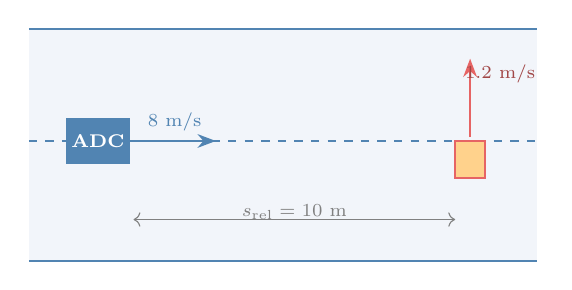
\begin{tikzpicture}[scale=0.95, transform shape]
  \fill[bglight] (0,-1.3) rectangle (6.8,1.8);
  \draw[deepblue, thick] (0,-1.3) -- (6.8,-1.3);
  \draw[deepblue, thick] (0, 1.8) -- (6.8, 1.8);
  \draw[deepblue, dashed, thin] (0,0.3) -- (6.8,0.3);

  \fill[egopt] (0.5,0) rectangle (1.35,0.6);
  \node[white, font=\scriptsize\bfseries] at (0.925,0.3) {ADC};
  \draw[-Stealth, thick, deepblue] (1.4,0.3) -- (2.5,0.3);
  \node[font=\scriptsize, deepblue] at (1.95,0.55) {8 m/s};

  \fill[obsdyn] (5.7,-0.2) rectangle (6.1,0.3);
  \draw[-Stealth, thick, dangerred] (5.9,0.35) -- (5.9,1.4);
  \node[font=\scriptsize, dangerred!70!black] at (6.3,1.2) {1.2 m/s};

  \draw[<->, thin, gray] (1.4,-0.75) -- (5.7,-0.75);
  \node[font=\scriptsize, gray] at (3.55,-0.65) {$s_{\text{rel}}=10$ m};
\end{tikzpicture}
}
  \caption{$t{=}0$ 行人未进入路径}
\end{subfigure}\hfill
\begin{subfigure}[b]{0.32\textwidth}
  \centering
  \adjustbox{max width=\linewidth}{% 动态障碍物排除 t=0.625s（子图 b）
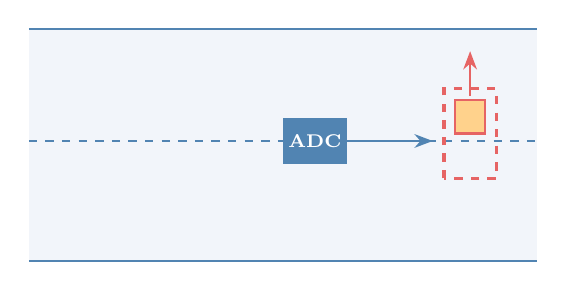
\begin{tikzpicture}[scale=0.95, transform shape]
  \fill[bglight] (0,-1.3) rectangle (6.8,1.8);
  \draw[deepblue, thick] (0,-1.3) -- (6.8,-1.3);
  \draw[deepblue, thick] (0, 1.8) -- (6.8, 1.8);
  \draw[deepblue, dashed, thin] (0,0.3) -- (6.8,0.3);

  \fill[egopt] (3.4,0) rectangle (4.25,0.6);
  \node[white, font=\scriptsize\bfseries] at (3.825,0.3) {ADC};
  \draw[-Stealth, thick, deepblue] (4.3,0.3) -- (5.4,0.3);

  \fill[obsdyn] (5.7,0.4) rectangle (6.1,0.85);
  \draw[-Stealth, thick, dangerred] (5.9,0.9) -- (5.9,1.5);

  \draw[dangerred, very thick, dashed] (5.55,-0.2) rectangle (6.25,1.0);
\end{tikzpicture}
}
  \caption{中间时刻行人半入路径}
\end{subfigure}\hfill
\begin{subfigure}[b]{0.32\textwidth}
  \centering
  \adjustbox{max width=\linewidth}{% 动态障碍物排除 t=1.25s（子图 c）
\begin{tikzpicture}[scale=0.95, transform shape]
  \fill[bglight] (0,-1.3) rectangle (6.8,1.8);
  \draw[deepblue, thick] (0,-1.3) -- (6.8,-1.3);
  \draw[deepblue, thick] (0, 1.8) -- (6.8, 1.8);
  \draw[deepblue, dashed, thin] (0,0.3) -- (6.8,0.3);

  \fill[egopt, opacity=0.3] (0.5,0) rectangle (1.35,0.6);
  \node[gray, font=\scriptsize] at (0.925,0.3) {$t=0$};

  \fill[egopt] (5.7,0) rectangle (6.55,0.6);
  \node[white, font=\scriptsize\bfseries] at (6.125,0.3) {ADC};

  \fill[obsdyn] (5.7,1.3) rectangle (6.1,1.75);
  \node[font=\scriptsize, dangerred!70!black, above] at (5.9,1.8) {已穿过};

  \fill[bandok] (1.5,0.05) rectangle (5.6,0.55);
  \node[font=\scriptsize, lightgreen!50!black] at (3.5,0.3) {路径已打开};
\end{tikzpicture}
}
  \caption{自车到达时通行带打开}
\end{subfigure}
\caption{横穿行人场景下的时间盲信息断裂}
\caption*{全时刻并集投影把行人扫过的整段车道并入静止足迹，路径层据此判定阻塞；而沿到达时间 $\tau(s)$ 的时变投影只取自车实际到达时刻的占用，通行带早已打开。}
\label{fig:dynamic_exclusion}
\end{figure}

\subsection{解耦可行域是联合可行域的子集}
\label{subsec:feasibility_subset}

把联合规划在三维时空中的可行轨迹集合记为 $\mathcal{F}_{joint}$，它由含时间维度的约束与运动学约束共同界定，自车的横向选择可以随时变约束协同调整。解耦规划分两步进行，路径子问题先在不含时间的约束下确定横向边界，速度子问题再在固定路径上调整速度，两层互不回溯。于是解耦可达的轨迹集合 $\mathcal{F}_{dec}$ 可写成路径可行域与其上条件速度可行域的顺序复合，路径分量先在式~\eqref{eq:prob_union} 的时间无关足迹约束下确定，速度分量再在已固定的路径几何上求解，并非两个独立集合的笛卡尔积，而是后者依赖前者的分层结构。由于任一解耦可行轨迹同时满足联合问题的约束，而联合问题允许的时变协同在解耦中被禁止，二者满足包含关系
\begin{equation}
    \mathcal{F}_{dec} \subseteq \mathcal{F}_{joint}.
    \label{eq:prob_subset}
\end{equation}
当路径层以并集投影或 $t{=}0$ 静态快照取代时变投影时，路径可行域被进一步收缩，包含关系可退化为真子集 $\mathcal{F}_{dec} \subsetneq \mathcal{F}_{joint}$，由此出现解耦不可行而联合可行的情形。横穿行人即为一例，静态投影下路径层判定 BLOCKED，而沿 $\tau(s)$ 利用时变投影后中心间隙打开，路径重新可行。

\subsection{纯解耦不可行性的充分条件}
\label{subsec:infeasibility_condition}

解耦失效来自两个相互独立的机制，一是空间维度上逐障碍物贪心选向，二是时间维度上的静态投影。Baseline 在 \texttt{PathBoundsDeciderUtil} 中逐障碍物按其中心与参考值的相对位置独立判定绕行方向，决策一旦在循环中做出便不可回退，更新后若某截面 $l^{+}(s) < l^{-}(s)$ 即判定 BLOCKED，调用 \texttt{TrimPathBounds} 截断路径并触发 FallbackPath 停车。该贪心策略在 $2^k$ 种方向组合中仅检查其中一种，$k$ 为该截面活跃障碍物数。这两个机制各自给出纯解耦输出 BLOCKED 的一个充分条件，其形式化陈述与证明在第\ref{sec:theory}节给出，此处只作机理说明。

时间维度上，当动态障碍物的全时刻并集投影在某纵向区间上覆盖了去除半车宽后的整段可行区间时，时间盲的路径子问题在该区间无宽度足够的通行带，而沿到达时间 $\tau(s)$ 的时变投影下通行带仍可能为正，该充分条件由命题\ref{prop:decoupled_infeasible}刻画。空间维度上，逐障碍物贪心可能选中分裂式组合而遗漏可行解，而遍历全部 $k+1$ 个候选分割的最大间隙策略不会输出此类虚假 BLOCKED，这一点由定理\ref{thm:max_gap}保证。两个条件均为充分而非必要，贪心选向在多数场景与全局最优一致，仅在特定对称或密集配置下选中不可行组合，对两障碍物的四种方向组合而言只有 RL、LR 两种可能不可行。需要厘清逻辑方向。给定到达时间 $\tau(s)$ 后，当全部 $k+1$ 个候选分割在该截面均给出非正间隙时，该截面对应真实阻塞，这是触发 BLOCKED 的一个充分条件；反过来 Baseline 输出 BLOCKED 并不蕴含联合问题不可行，它也可能由时间盲的静态投影或贪心选中分裂式组合所造成的虚假阻塞触发。换言之，BLOCKED 是真实联合不可行的必要表现而非充分判据，其失效本质是解耦可行域 $\mathcal{F}_{dec}$ 相对 $\mathcal{F}_{joint}$ 的真子集收缩，既来自空间维度遗漏的可行组合，也来自时间维度抹除的时变窗口。

上述分析表明，Baseline 的次优性沿安全裕度、空间协调与时间投影三个维度展开，其共同根源在于解耦接口处的信息断裂，即统一安全裕度、逐障碍物独立决策与全时刻并集投影使路径层既缺乏分级机制又缺乏全局与时间视角。MIKU 不另起联合规划，而是在这一接口处建立显式约束传递通道，由表~\ref{tab:prob_channel} 所列三个组件分别回答传哪些信息、空间约束怎么传、时间约束怎么传，方法构造与理论保证在后续各节展开。

\begin{table}[htbp]
\centering
\caption{解耦失效的三个维度与 MIKU 显式约束传递通道的对应}
\label{tab:prob_channel}
\begin{tabular}{p{2.4cm} p{4.6cm} p{4.6cm}}
\hline
失效维度 & 解耦接口处的断裂 & 通道组件的回答 \\
\hline
安全裕度 & 所有障碍物共用统一 $\delta$，低威胁障碍物压缩通行带 & 传哪些，多因子威胁度过滤给出差异化裕度 $\delta_i$ \\
空间协调 & 逐障碍物独立贪心选向，遗漏可行的全局组合 & 空间怎么传，扫描线分组与组级最大间隙通行带 \\
时间投影 & 全时刻并集或 $t{=}0$ 快照抹除预测轨迹 & 时间怎么传，$\tau(s)$ 时变投影构造时空可通行走廊注入速度 QP \\
\hline
\end{tabular}
\end{table}

% ====== _parts/method.tex ======

\section{MIKU 方法与显式约束传递通道}
\label{sec:method}

第\ref{sec:problem}节已经表明，Apollo 路径--速度解耦架构的瓶颈不在于某个模块的参数整定，而在于两个阶段之间的接口本身丢弃了时间维度，路径阶段只看 $t=0$ 的静态快照，速度阶段拿到一条已经固定的路径后只能被动制动。多障碍物交互运动学统一规划算法（Multi-obstacle Interaction-density Kinematic-prediction Unified planner, MIKU）不重写这一架构，而是在解耦接口处建立一条显式的约束传递通道，让路径阶段已经掌握的安全与时序信息能够完整地抵达速度阶段。

这条通道需要回答三个问题，本节的三个组件分别对应其中之一。其一是传递什么，即把 Apollo 一刀切的安全裕度替换为按威胁程度分级的差异化裕度 $\delta_i$，使真正危险的障碍物得到不低于原方案的保护，低威胁障碍物则归还被无谓占用的横向空间。其二是横向信息如何传递，即在单个纵向截面上把多障碍物的避让决策从逐个独立的贪心改为组级协调，以一次线性扫描求出全局最优的通行带。其三是时间信息如何传递，即以到达时间函数 $\tau(s)$ 为桥梁，把动态障碍物的预测轨迹投影到自车实际到达时刻的横向位置，构造时空可通行走廊，并经 \texttt{STDrivableBoundary} 把走廊约束注入速度二次规划（Quadratic Programming, QP）。三个组件不是三项并列的贡献，而是同一条通道上前后衔接的三段，它们共享统一的安全边界记号 $u_i$、$v_i$ 并复用同一套间隙最优性结论。整体数据流如图~\ref{fig:algorithm_flow} 所示。

\begin{figure}[htbp]
\centering
\adjustbox{max width=\textwidth}{% MIKU 多障碍物统一规划算法总流程
\begin{tikzpicture}[
    scale=1.0, transform shape,
    stepimp/.style={rectangle, rounded corners=3pt, draw=deeppink, fill=improvedpink, minimum width=5.4cm, minimum height=1.0cm, font=\small, align=center},
    inp/.style={rectangle, draw=deepblue, fill=inputyellow, minimum width=4.0cm, minimum height=0.8cm, font=\footnotesize, align=center},
    outnode/.style={rectangle, rounded corners=3pt, draw=deeppink, fill=outputpink, minimum width=4.0cm, minimum height=0.8cm, font=\small\bfseries, align=center},
    qpnode/.style={rectangle, rounded corners=3pt, draw=deepblue, fill=lightblue, minimum width=4.0cm, minimum height=0.8cm, font=\small\bfseries, align=center},
    arr/.style={-Stealth, thick, deepblue},
    injarr/.style={-Stealth, thick, deeppink},
]

% 输入
\node[inp] (i1) at (-5.8, 6.0) {参考线 $+$ 障碍物集合};
\node[inp] (i2) at (-5.8, 5.0) {预测轨迹 $+$ 车辆状态};

% 步骤（间距 1.7，全部为 MIKU 改进）
\node[stepimp] (s1) at (0, 5.5)  {\textbf{Step 1} 到达时间 $\tau(s)$ 与时变 SL 投影};
\node[stepimp] (s2) at (0, 3.8)  {\textbf{Step 2} 多因子威胁度评估 $\Theta_i$};
\node[stepimp] (s3) at (0, 2.1)  {\textbf{Step 3} 动态安全裕度 $\delta_i$ 与边界 $u_i,v_i$};
\node[stepimp] (s4) at (0, 0.4)  {\textbf{Step 4} 扫描线重叠分组 $\mathcal{G}_1,\ldots,\mathcal{G}_m$};
\node[stepimp] (s5) at (0,-1.3)  {\textbf{Step 5} 组内最大间隙 $g^\star_j=\max_k g_{j,k}$};
\node[stepimp] (s6) at (0,-3.0)  {\textbf{Step 6} 合并全局路径横向边界};
\node[stepimp] (s7) at (0,-4.7)  {\textbf{Step 7} ST 时空可通行走廊 $\Omega$};

% 输出（左侧）与跨接口的速度 QP
\node[outnode] (o1) at (-5.8,-3.0) {路径横向边界};
\node[outnode] (o2) at (-5.8,-4.7) {时空可通行走廊};
\node[qpnode]  (qp) at (-5.8,-6.4) {速度 QP（求解器不变）};

% 输入箭头
\draw[arr] (i1.east) -- (s1.west);
\draw[arr] (i2.east) -- (s1.west);

% 步骤间箭头
\draw[arr] (s1) -- (s2);
\draw[arr] (s2) -- (s3);
\draw[arr] (s3) -- (s4);
\draw[arr] (s4) -- (s5);
\draw[arr] (s5) -- (s6);
\draw[arr] (s6) -- (s7);

% 输出箭头
\draw[arr] (s6.west) -- (o1.east);
\draw[arr] (s7.west) -- (o2.east);

% 走廊注入速度 QP（跨解耦接口）
\draw[injarr] (o2.south) -- node[right, font=\footnotesize, deeppink] {逐时间步纵向上界} (qp.north);

\end{tikzpicture}
}
\caption{MIKU 显式约束传递通道的整体数据流}
\caption*{威胁度过滤输出差异化裕度，扫描线分组与组级最大间隙在 SL 层求出最优通行带，到达时间函数构造时空走廊并经 \texttt{STDrivableBoundary} 注入速度 QP，路径 QP 与速度 QP 的内部求解结构保持不变。}
\label{fig:algorithm_flow}
\end{figure}

\subsection{多因子威胁度与差异化安全裕度}
\label{sec:method_threat}

Apollo 的路径边界构建环节由 \texttt{PathBoundsDeciderUtil} 的静态方法承载，其 \texttt{GetBufferBetweenADCCenterAndEdge} 对所有障碍物返回同一套安全裕度，即半车宽再加固定的额外缓冲 \texttt{obstacle\_lat\_buffer}，不区分障碍物的类型、速度与横向偏移。其上仅有的分级来自障碍物侧向 nudge 判定以 $0.5$\,m/s 速度阈值所做的静态与非静态二分，由 \texttt{static\_obstacle\_nudge\_l\_buffer} 与 \texttt{nonstatic\_obstacle\_nudge\_l\_buffer} 两个独立参数控制，静态障碍物取 $0.3$\,m、非静态取 $0.4$\,m，与前述 \texttt{obstacle\_lat\_buffer} 分属不同参数、走不同代码路径。这一粒度既无法区分轨迹突变的行人与可预测的同向车辆，也无法区分正面逼近与横向远离的障碍物。在窄路场景中，统一缓冲会把两侧净间距同时压到小于车宽，使路径边界构建输出零宽通行带而判定 BLOCKED。

MIKU 以一个归一化的威胁度 $\Theta_i$ 取代上述二分，对每个障碍物综合 5 个因子加权得到

\begin{equation}
    \Theta_i = w_1 f_{TTC}(i) + w_2 f_{overlap}(i) + w_3 f_{vel}(i) + w_4 f_{type}(i) + w_5 f_{inter}(i),
    \label{eq:threat_score}
\end{equation}

其中各因子均归一化至 $[0,1]$，权重之和为一，故 $\Theta_i \in [0,1]$。权重取 $w_1=0.30$、$w_5=0.25$、$w_2=0.20$、$w_3=0.15$、$w_4=0.10$，呈 $w_1>w_5>w_2>w_3>w_4$ 的次序。该次序先依据各因子对多障碍物场景风险的区分度做定性排序，再在对称路锥与横穿行人等典型场景上核对威胁度排序是否符合驾驶直觉后微调确定。碰撞时间与交互密度对场景风险的区分度最高，赋予较大权重；障碍物类型在同一场景内变化较小，赋予较小权重。

5 个因子各刻画一种风险来源。碰撞时间（Time To Collision, TTC）因子衡量纵向碰撞的紧迫性，

\begin{equation}
    \mathrm{TTC}_i =
    \begin{cases}
        \dfrac{s_i - s_{ego}}{\dot{s}_{ego} - \dot{s}_i}, & s_i > s_{ego} \ \text{且}\ \dot{s}_{ego} > \dot{s}_i, \\[0.6em]
        +\infty, & \text{其它},
    \end{cases}
    \label{eq:ttc}
\end{equation}

障碍物位于自车后方、自车不会追上或相对速度为零等退化情形均令 $\mathrm{TTC}_i=+\infty$，不构成纵向威胁。再以分段线性映射

\begin{equation}
    f_{TTC}(i) =
    \begin{cases}
        1, & \mathrm{TTC}_i \leq T_{crit}, \\[0.3em]
        \dfrac{T_{max} - \mathrm{TTC}_i}{T_{max} - T_{crit}}, & T_{crit} < \mathrm{TTC}_i < T_{max}, \\[0.6em]
        0, & \mathrm{TTC}_i \geq T_{max},
    \end{cases}
    \label{eq:f_ttc}
\end{equation}

把碰撞时间转为威胁度，临界值取 $T_{crit}=2.0$\,s，依据 Minderhoud 与 Bovy 对碰撞时间分布的分析，碰撞时间低于该值时驾驶员已难以靠转向规避；上限取 $T_{max}=7.0$\,s，与 Apollo ST 图的时间视野一致。

其余四个因子分别从横向、速度、类型与密集度补全风险画像。横向重叠率因子 $f_{overlap}(i)=\max\!\big(0,\ \min(l_i^{+}, l_{ego}^{+}) - \max(l_i^{-}, l_{ego}^{-})\big)/W_{ego}$ 度量障碍物与自车走廊在横向上的重叠比例，零表示完全错开、一表示正对自车。相对速度因子 $f_{vel}(i)=\sigma(v_{rel,i}/v_{max})$ 采用 $\sigma(x)=1/(1+e^{-5x})$ 的 Sigmoid 映射，$v_{rel,i}=\dot{s}_{ego}-\dot{s}_i$，选择 Sigmoid 而非线性是因为相对速度过零附近的区分更重要，而极高相对速度之间无需精细区分。类型因子 $f_{type}(i)$ 取离散值，综合运动不确定性与事故后果，行人、骑行者等弱势道路使用者（Vulnerable Road User, VRU）取 $1.0$，机动车取 $0.7$，未知可动目标取 $0.5$，静态障碍物取 $0.3$，交通锥等小尺寸标识物取 $0.15$，其中 VRU 在同等碰撞能量下受伤与致死风险远高于车内乘员，因而施加额外保护。交互密度因子

\begin{equation}
    f_{inter}(i) = \frac{1}{N-1} \sum_{j \neq i} \mathbf{1}\!\left[d_{ij} < d_{cluster}\right] \cdot \frac{d_{cluster} - d_{ij}}{d_{cluster}},
    \label{eq:f_inter}
\end{equation}

以 SL 平面欧氏距离 $d_{ij}$ 与聚类半径 $d_{cluster}=10$\,m 加权统计邻近障碍物的聚集程度，孤立障碍物 $f_{inter}\approx 0$，密集车群中接近 $1$，$N=1$ 时令 $f_{inter}=0$。交互密度高的障碍物通常落入同一连通分量，将在第\ref{sec:method_band}节的纵向重叠分组中被统一协调。

威胁度确定后，把额外缓冲在区间 $[d_{buf,min}, d_{buf,max}]$ 上随威胁度线性插值，再加半车宽合成最终安全裕度

\begin{equation}
    d_{buf,i} = d_{buf,min} + (d_{buf,max} - d_{buf,min})\,\Theta_i, \qquad
    \delta_i = \frac{W_{ego}}{2} + d_{buf,i},
    \label{eq:dynamic_delta}
\end{equation}

额外缓冲区间取 $[0.10, 0.40]$\,m。式\eqref{eq:dynamic_delta}在两个端点上保持安全语义。$\Theta_i \to 1$ 时额外缓冲达到 $0.40$\,m，总裕度与 Apollo 原方案相同或更大，安全性不下降；$\Theta_i \to 0$ 时额外缓冲降至 $0.10$\,m，总裕度仍含完整的 $W_{ego}/2$，仅把原本被无谓占用的横向空间归还给通行带。当所有 $\Theta_i$ 取同一值时，式\eqref{eq:dynamic_delta}退化为统一缓冲方案。差异化裕度随即改写每个障碍物的横向安全边界

\begin{equation}
    u_i = l_i^{-} - \delta_i, \qquad v_i = l_i^{+} + \delta_i,
    \label{eq:dynamic_uv}
\end{equation}

其中 $u_i$ 是自车从右侧通过该障碍物时参考点横向坐标的上界，$v_i$ 是从左侧通过时的下界。差异化的 $\delta_i$ 只改变 $u_i$、$v_i$ 的取值，不破坏第\ref{sec:method_band}节引理与定理对 $u$ 值排序性的依赖，下游的组级最优性结论原样成立。

\subsection{扫描线分组与组级最大间隙通行带}
\label{sec:method_band}

确定了每个障碍物的安全边界之后，第二个问题是如何在横向上把这些约束传递成一条全局协调的通行带。Apollo 的路径边界构建在 \texttt{PathBoundsDeciderUtil} 的 \texttt{UpdatePathBoundaryBySLPolygon} 中逐障碍物决定 LEFT\_NUDGE 或 RIGHT\_NUDGE，不考虑同一 $s$ 截面上其余活跃障碍物。两侧同时存在障碍物时，左侧障碍物下压上边界、右侧障碍物上抬下边界，容易出现 $l^{+}(s)<l^{-}(s)$，路径边界判 BLOCKED 后由 \texttt{TrimPathBounds} 截断并触发 \texttt{FallbackPath} 停车。$k$ 个障碍物同时活跃时避让方向共有 $2^k$ 种组合，贪心仅检查其中一种，可能恰好选中不可行组合而错过可行解，这种失效集中出现在对称或密集配置。MIKU 把单截面问题整理为按安全边界排序后的间隙选择问题，并先按纵向重叠把障碍物分组，使彼此无关的障碍物分别独立求解。

两个障碍物 $O_i$ 与 $O_j$ 称为纵向重叠，当且仅当各自纵向占据区间满足 $[s_i^{-}, s_i^{+}] \cap [s_j^{-}, s_j^{+}] \neq \varnothing$。该关系对称但不传递。取其传递闭包，把 $n$ 个障碍物划为 $m$ 个连通分量 $C_1, \ldots, C_m$，不同分量的纵向区间并集互不相交，任意 $s$ 截面至多受一个分量影响，分量间的避让决策可独立求解。分组用一次扫描线完成，按 $s_i^{-}$ 升序排列后维护当前分量已见的最大 $s^{+}$ 记为 $s_{max}$，若下一障碍物的 $s^{-}$ 不超过 $s_{max}$ 则并入当前分量并更新 $s_{max}$，否则另起新分量。排序为 $O(n\log n)$，扫描本身 $O(n)$，分组总体 $O(n\log n)$。

连通分量不保证存在所有成员共同活跃的公共截面，链式情形中 $O_1$ 与 $O_2$ 重叠、$O_2$ 与 $O_3$ 重叠，而 $O_1$ 与 $O_3$ 可能完全错开。对链式分量取保守包络处理，把同一分量内所有障碍物视为同时施加约束，在其覆盖区间上取所有 $u_i$ 的最小值与所有 $v_i$ 的最大值。由于任一真实截面的活跃集合都是分量的子集，包络宽度是真实通行带宽度的下界，包络宽度不小于车宽即保证该分量内所有截面均可通行；包络不可行只说明充分条件不成立，并不意味着真实场景必然阻塞。这一处理保证安全，但不声称对一般链式分量给出全局最优。全路径的通行带宽度由最窄分量决定，

\begin{equation}
    \hat{W} = \min_{j=1,\ldots,m} \hat{W}(C_j).
    \label{eq:global_width}
\end{equation}

在单个分量内部，单截面最优分割具有可一次扫描求解的结构，本节给出其构造，形式化陈述与证明集中在第\ref{sec:theory}节。第一步压缩搜索空间。把分量内 $k$ 个障碍物按 $u_i$ 值升序排列后，最优避让方向必呈连续分割，即存在分割点 $p\in\{0,1,\ldots,k\}$ 使排序后前 $p$ 个左绕、后 $k-p$ 个右绕，由此 $2^k$ 个任意方向组合被压缩为 $k+1$ 个候选分割，这一连续性由引理\ref{lem:continuous_partition}保证。其中 $p=0$ 表示全部右绕、自车走最右侧通道，$p=k$ 表示全部左绕、自车走最左侧通道，$1\leq p\leq k-1$ 表示自车从第 $p$ 与第 $p+1$ 个障碍物之间的间隙通过。存在 $u_i$ 相同的障碍物时以 $v_i$ 降序作二级排序键保证唯一性。

第二步把每个候选分割的通行带宽度归约为一个几何间隙。仅按 $u_i$ 排序不保证 $v_i$ 单调，故引入前缀左安全边界 $V_p=\max_{1\leq q\leq p} v_{(q)}$，并对 $p=0,1,\ldots,k$ 定义 $k+1$ 个间隙 $g_p$，其中 $g_0$ 是道路右边界到最右侧障碍物的间隙，$g_k$ 是前 $k$ 个障碍物形成的最左安全边界到道路左边界的间隙，中间的 $g_p$ 是前 $p$ 个障碍物的最左安全边界 $V_p$ 与后续障碍物最右安全边界 $u_{(p+1)}$ 之间的间隙，其精确表达见式\eqref{eq:gap_def}。障碍物横向边界不交错时 $V_p=v_{(p)}$，该定义退化为相邻障碍物之间的普通几何间隙。在所有障碍物的安全裕度扩展未越出道路边界的前提下，分割点 $p$ 对应的通行带宽度恰等于 $g_p$，最优通行带宽度为 $W^{*}=\max_{p} g_p$，即取最大间隙对应的分割点为最优解，这一最大间隙最优性由定理\ref{thm:max_gap}给出。当某障碍物膨胀后越出道路边界时，先按引理\ref{lem:boundary_trim}的越界预处理规则强制其避让方向并移出候选列表，使定理前提成立。

几个边界情形可被算法自然吸收。其一，当 $V_p>u_{(p+1)}$ 时 $g_p<0$，该通道不可通行，扫描比较时被自动跳过。其二，当全部 $k+1$ 个间隙都不足车宽，即 $\max_p g_p < W_{ego}$，说明该截面无可通行路径，这是真实 BLOCKED 而非算法局限。所有 $u_i$、$v_i$ 均按差异化裕度 $\delta_i$ 计算，引理与定理仅依赖 $u$ 值排序性而不依赖 $\delta_i$ 是否为常数，故第\ref{sec:method_threat}节的差异化裕度与本节的最优性结论彼此兼容。单截面经排序加一次扫描求解，复杂度由暴力枚举的 $O(2^k)$ 降为 $O(k\log k)$。

\begin{figure}[htbp]
\centering
\begin{subfigure}[b]{0.46\textwidth}
  \centering
  \adjustbox{max width=\linewidth}{% 贪心独立决策 → BLOCKED（子图 a）
\begin{tikzpicture}[scale=0.85, transform shape]
  % 道路
  \fill[bglight] (-0.5,-2.5) rectangle (8.5,2.5);
  \draw[gray, thick] (-0.5, 2.5) -- (8.5, 2.5);
  \draw[gray, thick] (-0.5,-2.5) -- (8.5,-2.5);
  \draw[dashed, gray!60] (-0.5, 0) -- (8.5, 0);
  \node[gray, font=\scriptsize, anchor=east] at (-0.6, 0) {$l{=}0$};

  % O_a（上方靠边）y=[0.5, 1.0]
  \fill[dangerred!70, draw=dangerred, thick] (3.2, 0.5) rectangle (4.8, 1.0);
  \node[font=\scriptsize, white] at (4.0, 0.75) {$O_a$};

  % O_b（下方靠边）y=[-1.0, -0.5]
  \fill[dangerred!70, draw=dangerred, thick] (3.2,-1.0) rectangle (4.8,-0.5);
  \node[font=\scriptsize, white] at (4.0,-0.75) {$O_b$};

  % 膨胀虚线 δ=0.4
  \draw[dangerred!60, dashed, thick] (2.8, 0.1) rectangle (5.2, 1.4);
  \draw[dangerred!60, dashed, thick] (2.8,-1.4) rectangle (5.2,-0.1);

  % 决策标注
  \node[deepblue, font=\scriptsize\bfseries] at (5.5, 0.75) {R};
  \node[deeppink, font=\scriptsize\bfseries] at (2.5,-0.75) {L};

  % 独立决策：O_a 右绕 → 上界压到 0.1-0.1=0.0
  %           O_b 左绕 → 下界抬到 -0.1+0.1=0.0
  % l+ ≈ l- → BLOCKED

  % 上界 l+(s) 凹字形（offset 区分）
  \draw[deeppink, very thick]
    (-0.5, 2.5) -- (2.6, 2.5) -- (2.6, 0.0) -- (5.4, 0.0) -- (5.4, 2.5) -- (8.5, 2.5);
  \node[deeppink, font=\scriptsize] at (7.5, 2.1) {$l^+(s)$};

  % 下界 l-(s) 凸字形
  \draw[deepblue, very thick]
    (-0.5,-2.5) -- (2.6,-2.5) -- (2.6, 0.0) -- (5.4, 0.0) -- (5.4,-2.5) -- (8.5,-2.5);
  \node[deepblue, font=\scriptsize] at (7.5,-2.1) {$l^-(s)$};

  % BLOCKED 标注
  \node[dangerred, font=\scriptsize\bfseries] at (4.0, 1.8) {$l^+ \leq l^-$ $\Rightarrow$ BLOCKED};

  % 自车
  \fill[deepblue, opacity=0.4] (0.3,-0.3) rectangle (1.8,0.3);
  \draw[deepblue, thick, rounded corners=1pt] (0.3,-0.3) rectangle (1.8,0.3);
  \node[deepblue, font=\tiny\bfseries] at (1.05,0) {自车};
\end{tikzpicture}
}
  \caption{逐障碍物贪心分裂式选向}
\end{subfigure}\hfill
\begin{subfigure}[b]{0.46\textwidth}
  \centering
  \adjustbox{max width=\linewidth}{% 全局协调统一右绕 → 通行（子图 b）
\begin{tikzpicture}[scale=0.85, transform shape]
  % 道路
  \fill[bglight] (-0.5,-2.5) rectangle (8.5,2.5);
  \draw[gray, thick] (-0.5, 2.5) -- (8.5, 2.5);
  \draw[gray, thick] (-0.5,-2.5) -- (8.5,-2.5);
  \draw[dashed, gray!60] (-0.5, 0) -- (8.5, 0);
  \node[gray, font=\scriptsize, anchor=east] at (-0.6, 0) {$l{=}0$};

  % O_a（上方靠边）y=[0.5, 1.0]
  \fill[dangerred!70, draw=dangerred, thick] (3.2, 0.5) rectangle (4.8, 1.0);
  \node[font=\scriptsize, white] at (4.0, 0.75) {$O_a$};

  % O_b（下方靠边）y=[-1.0, -0.5]
  \fill[dangerred!70, draw=dangerred, thick] (3.2,-1.0) rectangle (4.8,-0.5);
  \node[font=\scriptsize, white] at (4.0,-0.75) {$O_b$};

  % 膨胀虚线 δ=0.4（统一右绕）
  \draw[dangerred!60, dashed, thick] (2.8, 0.1) rectangle (5.2, 1.4);
  \draw[dangerred!60, dashed, thick] (2.8,-1.4) rectangle (5.2,-0.1);

  % 决策标注（统一 R）
  \node[deepblue, font=\scriptsize\bfseries] at (5.5, 0.75) {R};
  \node[deepblue, font=\scriptsize\bfseries] at (5.5,-0.75) {R};

  % 统一右绕 → 上界压到 O_b 膨胀下缘 -1.4（offset -0.1）
  \draw[deeppink, very thick]
    (-0.5, 2.5) -- (2.6, 2.5) -- (2.6, -1.5) -- (5.4, -1.5) -- (5.4, 2.5) -- (8.5, 2.5);
  \node[deeppink, font=\scriptsize] at (7.5, 2.1) {$l^+(s)$};

  % 下界保持道路下界
  \draw[deepblue, very thick, dashed]
    (-0.5,-2.5) -- (8.5,-2.5);
  \node[deepblue, font=\scriptsize, left] at (-0.6,-2.5) {$l^-(s)$};

  % 通行带
  \fill[lightgreen, opacity=0.25] (-0.5,-2.5) rectangle (8.5,-1.5);

  % 通行带宽度
  \draw[lightgreen!60!black, thick, {Stealth}-{Stealth}] (0.5,-2.5) -- (0.5,-1.5);
  \node[lightgreen!60!black, font=\scriptsize, anchor=east] at (0.4,-2.0) {$W{=}1.0$m};

  % 自车轨迹（无 fill）
  \draw[deepblue, very thick, -{Stealth}]
    plot[smooth, tension=0.55] coordinates
      {(0.5, 0) (1.5,-0.5) (2.5,-1.8) (4.0,-2.0) (5.5,-1.8) (6.5,-0.5) (7.5, 0)};
  \node[deepblue, font=\scriptsize] at (4.0,-2.4) {规划轨迹};

  % PASS 判定
  \node[draw=lightgreen!80!black, fill=lightgreen!20, font=\scriptsize,
        rounded corners=3pt] at (4.0, 2.0)
    {统一右绕 $\Rightarrow$ \textbf{PASS}};
\end{tikzpicture}
}
  \caption{组级最大间隙统一选向}
\end{subfigure}
\caption{两个近似对称障碍物下贪心选向与组级最优的差异}
\caption*{贪心对两障碍物分别独立选向，从两侧同时收缩边界把自车挤入中间窄缝而判定阻塞；遍历 $k{+}1$ 个候选分割的最大间隙策略选中统一绕行，借另一侧充裕空间通过。}
\label{fig:greedy_vs_global}
\end{figure}

\subsection{到达时间函数与时空可通行走廊}
\label{sec:method_corridor}

前两个组件都在 $t=0$ 的静态截面上工作。第三个组件回答时间信息如何传递，把横向通行性沿时间轴推广到动态障碍物，并跨过解耦接口抵达速度规划。其桥梁是到达时间函数 $\tau(s)$，给出自车抵达纵向位置 $s$ 的预估时刻。强调 $\tau(s)$ 在路径阶段是给定参数而非优化变量，由二阶运动学模型或上周期速度曲线估计，路径阶段的决策变量仍只是方向组合。以匀加速运动学估计时

\begin{equation}
    \tau(s) = \frac{-v_{ego} + \sqrt{v_{ego}^{2} + 2\,a_{ego}\,(s - s_{ego})}}{a_{ego}},
    \label{eq:arrival_time}
\end{equation}

其中 $s_{ego}$、$v_{ego}$、$a_{ego}$ 取自 \texttt{VehicleState}。$a_{ego}\to 0$ 时式\eqref{eq:arrival_time}经 Taylor 展开退化为匀速估计 $\tau(s)\approx (s-s_{ego})/v_{ego}$；$v_{ego}\approx 0$ 且 $a_{ego}\approx 0$ 时令 $\tau(s)=+\infty$，算法退回静态版本。当 $a_{ego}<0$ 即减速且根号内判别式 $v_{ego}^{2}+2a_{ego}(s-s_{ego})<0$ 时，表示自车在当前减速度下无法抵达 $s$，对应到达时刻不存在，此时同样令 $\tau(s)=+\infty$、按障碍物全时刻并集投影保守处理该截面，因此式\eqref{eq:arrival_time}始终取实数分支。实现上优先利用上周期速度曲线 $s_{prev}(t)$，若其单调不减则以一维查表加线性插值求首次满足 $s_{prev}(t)\geq s$ 的时刻，仅在无历史曲线、曲线非单调或查询越界时回退到式\eqref{eq:arrival_time}。单规划周期内的位置预测误差量级约为 $\tfrac{1}{2}a_{max}\Delta t^{2}$，远小于安全裕度区间 $[0.10, 0.40]$\,m，不对通行带边界判定构成实质影响。

有了 $\tau(s)$，每个动态障碍物的横向占据便取自其在自车到达时刻的预测位置。对障碍物 $i$，在 Prediction 模块给出的未来 $6$\,s 预测轨迹中查询时刻 $\tau(s)$ 的位置并线性插值，投影至参考线 Frenet 坐标得 $(s_i(\tau), l_i(\tau))$，结合几何尺寸得到时变 SL 边界 $[l_i^{-}(\tau(s)), l_i^{+}(\tau(s))]$；若该时刻障碍物纵向位置与 $s$ 的距离超过其纵向尺寸一半，则标记其在 $s$ 处不活跃。预测视野之外保守取最后预测位置不变。当前实现取概率最高的一条轨迹，扩展到多轨迹并集可降低漏判风险但查询次数线性增加。第\ref{sec:method_threat}节的横向重叠率因子同样改用该时变投影，即以 $f_{overlap}(i, \tau(s))$ 评估动态障碍物，静态障碍物仍取 $t=0$ 观测位置。

把第\ref{sec:method_band}节的静态间隙优化逐截面推广到动态情形。在每个 $s$ 截面按 $u_i(\tau(s))$ 排序后定义时变间隙

\begin{equation}
    g_p(s) =
    \begin{cases}
        u_{(1)}(\tau(s)) - l_{road}^{-}(s), & p=0, \\[0.3em]
        u_{(p+1)}(\tau(s)) - V_p(s), & p=1,\ldots,k-1, \\[0.3em]
        l_{road}^{+}(s) - V_k(s), & p=k,
    \end{cases}
    \label{eq:time_varying_gap}
\end{equation}

前缀左安全边界相应改为 $V_p(s)=\max_{1\leq q\leq p} v_{(q)}(\tau(s))$。引理\ref{lem:continuous_partition}与定理\ref{thm:max_gap}给出的是每个 $s$ 截面上的逐截面最优。把逐截面最优拼接为全路径解需要附加约束，本文沿用 Apollo 路径优化对单条参考线输出单一连续偏移曲线的工程约定，要求沿同一连通分量内固定同一组级分割。需要明确，这里固定的是各障碍物到左绕集合 $\mathcal{L}$ 与右绕集合 $\mathcal{R}$ 的指派，即每个障碍物全程同侧绕行，而非固定排序序号 $p$。当分量覆盖区间内各障碍物的 $u_i(\tau(s))$ 相对序不随 $s$ 翻转时，按 $u_i$ 升序的序号分割与左右指派分割一致，逐截面最优可拼接为下述受限最优；若相对序在某 $s$ 处翻转，则同一序号 $p$ 在不同截面对应不同障碍物指派，单条连续偏移曲线无法同时实现，此时退回保守包络处理，与链式分量同。在指派固定的前提下，该约束下的最优分割取使整段最薄截面最宽的极大极小解

\begin{equation}
    W^{*} = \max_{p}\ \min_{s}\ g_p(s),
    \label{eq:time_varying_opt}
\end{equation}

实现上仍以保守包络处理链式连通分量，保证安全可行但不声称全局最优。需要说明，式\eqref{eq:time_varying_opt}的极大极小解是固定单一分割约束下的受限最优，而非允许分割沿 $s$ 变化的无约束最优；逐截面最优的分割点 $p^{*}(s)$ 一般随 $s$ 变化，但单条连续偏移曲线无法实现分割沿程切换，故本文以单分割受限最优为工程上可实现的目标，定理\ref{thm:max_gap}的逐截面最优性在此约束下退化为对最薄截面的保证。选定最优分割 $p^{*}$ 后，把 SL 通行性沿 $\tau(s)$ 抬升至 ST 平面，得到时空可通行走廊

\begin{equation}
    \Omega = \left\{ (s,t) \ \middle|\ g_{p^{*}}(s) \geq W_{ego}\ \text{且}\ t \geq \tau(s) \right\}.
    \label{eq:st_corridor}
\end{equation}

走廊有两种几何特征。其一是禁行切片，若某 $s_k$ 处最优间隙不足车宽，整条纵向列 $\{s_k\}\times\mathbb{R}_{+}$ 被排除，在 $s$ 方向表现为水平缺口。其二是 $\tau(s)$ 左下沿，要求自车不早于 $\tau(s)$ 到达 $s$，为动态障碍物移开预留时间。两者组合使 $\Omega$ 在几何上是非凸集合。需要说明的是，方法的凸性来源不在 $\Omega$ 本身，而在其沿离散时间步的逐时间步线性投影 $s_j^{ub}$，这与 Baseline 经 \texttt{PathTimeHeuristicOptimizer} 在 $ST$ 图上动态规划粗搜索、再由 \texttt{SpeedDecider} 标定 YIELD/OVERTAKE 所得的线性盒约束在 QP 结构上一致，因而可在不改动速度求解器内部数据结构的前提下嵌入。

\begin{figure}[htbp]
\centering
\begin{subfigure}[b]{0.46\textwidth}
  \centering
  \adjustbox{max width=\linewidth}{% 图6(a) 车道汇入·Baseline：汇入车 ST 轨迹为倾斜平行四边形，
% 全时刻并集投影把其左沿保守压至 t=0，自车从起点即被挡，被迫停车。
\begin{tikzpicture}[scale=1.0, transform shape, arr/.style={-Stealth, thick}]
  \useasboundingbox (-0.75,-1.05) rectangle (5.85,4.75);

  % 汇入车 ST 轨迹：倾斜平行四边形，左沿压至 t=0（左下角 (0,1.2)）
  \fill[dangerred!35, draw=dangerred, thick]
    (0,1.2) -- (4.0,3.3) -- (4.0,4.3) -- (0,2.2) -- cycle;
  \node[font=\scriptsize\bfseries, dangerred!85!black, rotate=27] at (2.0,3.0) {汇入车 ST 轨迹};
  % 压至 t=0 标注
  \draw[dangerred, very thick] (0,1.2) -- (0,2.2);
  \node[font=\tiny, dangerred!80!black, anchor=east, align=right] at (-0.05,1.7) {左沿\\压至\\$t{=}0$};

  % 坐标轴
  \draw[arr] (0,0) -- (5.6,0) node[right, font=\scriptsize] {$t$/s};
  \draw[arr] (0,0) -- (0,4.5) node[above, font=\scriptsize] {$s$/m};
  \node[font=\tiny, left=2pt] at (0,0) {$0$};

  % Baseline s(t)：起步即撞平行四边形下沿，被迫停车（几乎不前进）
  \draw[deepblue, very thick, -Stealth]
    (0,0) .. controls (0.3,0.6) and (0.6,0.95) .. (0.8,1.0) -- (5.0,1.0);
  \fill[deepblue] (0.8,1.0) circle (1.6pt);
  \node[font=\tiny, deepblue!80!black, anchor=north] at (2.8,0.97) {自车被迫停车（无通行区）};
\end{tikzpicture}
}
  \caption{Baseline 时间盲投影}
\end{subfigure}\hfill
\begin{subfigure}[b]{0.46\textwidth}
  \centering
  \adjustbox{max width=\linewidth}{% 图6(b) 车道汇入·MIKU：按到达时间 τ(s) 摆放同一汇入车 ST 平行四边形，
% 其左沿右移至真实进入时刻，左下方让出三角通行区，自车得以争取一段前进。
\begin{tikzpicture}[scale=1.0, transform shape, arr/.style={-Stealth, thick}]
  \useasboundingbox (-0.75,-1.05) rectangle (5.85,4.75);

  % τ(s) 左下沿（楔形）：t≥τ(s) 可达
  \draw[deepblue, very thick, densely dashed] (0,0) -- (2.6,4.2);
  \node[font=\tiny, gray!55!black, align=center] at (0.55,3.75) {$t{<}\tau(s)$\\不可达};

  % 汇入车 ST 轨迹：同一平行四边形，左沿右移至 t=1.5（真实进入时刻）
  \fill[dangerred!35, draw=dangerred, thick]
    (1.5,1.2) -- (5.0,3.0) -- (5.0,4.0) -- (1.5,2.2) -- cycle;
  \node[font=\scriptsize\bfseries, dangerred!85!black, rotate=22] at (3.3,2.9) {汇入车 ST 轨迹};
  \draw[<-, dangerred!75!black, thin] (0.4,1.7) -- (1.45,1.7);
  \node[font=\tiny, dangerred!80!black, anchor=east, align=right] at (0.4,1.7) {左沿\\按 $\tau$\\右移};

  % 争取出的三角通行区（左下方）
  \fill[lightgreen!35] (0,0) -- (1.5,1.2) -- (1.5,0) -- cycle;
  \node[font=\tiny\bfseries, lightgreen!45!black, align=center] at (0.95,0.45) {通行区};

  % 坐标轴
  \draw[arr] (0,0) -- (5.6,0) node[right, font=\scriptsize] {$t$/s};
  \draw[arr] (0,0) -- (0,4.5) node[above, font=\scriptsize] {$s$/m};
  \node[font=\tiny, left=2pt] at (0,0) {$0$};

  % MIKU s(t)：沿通行区争取前进，随后与平行四边形下沿平行前进但保持间隙、不贴合
  \draw[deeppink, very thick, -Stealth]
    (0,0) .. controls (0.7,0.7) and (1.1,0.85) .. (1.4,0.9)
    .. controls (2.6,1.35) and (3.8,1.95) .. (5.0,2.45);
  \fill[deeppink] (1.4,0.9) circle (1.6pt);
  \node[font=\tiny, deeppink, anchor=north west] at (1.55,0.85) {争取前进后平行跟行};
  % 与下沿的间隙指示
  \draw[<->, gray!60, thin] (3.5,1.72) -- (3.5,2.28);
  \node[font=\tiny, gray!55!black, anchor=west] at (3.55,2.0) {间隙};
\end{tikzpicture}
}
  \caption{MIKU 时空可通行走廊 $\Omega$}
\end{subfigure}
\caption{ST 平面上的时空可通行走廊与上界收紧}
\caption*{Baseline 将动态障碍物全时刻并集压入禁行带；MIKU 沿 $\tau(s)$ 左下沿与禁行切片构造走廊 $\Omega$，逐时间步线性投影为速度变量的盒式上界注入 QP。}
\label{fig:corridor}
\end{figure}

\subsection{经 \texttt{STDrivableBoundary} 注入速度二次规划}
\label{sec:method_inject}

走廊只有进入速度求解器才能影响实际轨迹。走廊的有效性依赖自车实际到达时间不早于 $\tau(s)$，即对所有 $s$ 有 $t_{arrive}(s)\geq\tau(s)$，等价地写成速度约束 $s(t)\leq s_k$ 对所有 $t<\tau(s_k)$ 成立，含义是自车不得在 $\tau(s_k)$ 之前到达 $s_k$。该约束以收紧 QP 上界的方式注入。Apollo 的 \texttt{PiecewiseJerkSpeedOptimizer} 在等时间间隔 $\Delta t = 0.1$\,s 上以纵向位置 $s_j$、速度 $\dot{s}_j$、加速度 $\ddot{s}_j$ 为决策变量，此处 $0.1$\,s 为速度二次规划的时间离散步长，由速度优化配置决定，与 $100$\,ms 规划重规划周期分属两个量；目标函数惩罚跟踪误差与加加速度，约束含运动学等式约束、物理限制以及 \texttt{SpeedBoundsDecider} 给出的 ST 边界 $s_j^{lb,\mathrm{SBD}} \leq s_j \leq s_j^{ub,\mathrm{SBD}}$，整体写成

\begin{equation}
    \min_{\mathbf{x}}\ \tfrac{1}{2}\mathbf{x}^{\top}\mathbf{H}\mathbf{x} + \mathbf{f}^{\top}\mathbf{x}
    \quad \text{s.t.}\quad \mathbf{A}_{eq}\mathbf{x} = \mathbf{b}_{eq},\ \ \mathbf{x}^{lb} \leq \mathbf{x} \leq \mathbf{x}^{ub},
    \label{eq:qp_compact}
\end{equation}

由 OSQP 求解。每个动态障碍物取其 SL 投影首次进入候选走廊的纵向位置 $s_i^{0}$ 作为关键位置，连同对应到达时刻组成时间清单 $\mathcal{T} = \{(s_k, \tau_k)\}$，其规模等于动态障碍物数 $|\mathcal{D}|$，远小于时间步数 $K$。走廊约束随即对上界做一次收紧

\begin{equation}
    s_j^{ub} \leftarrow \min\!\left(s_j^{ub},\ s_k\right), \quad \forall\, j: t_j < \tau_k,\ \ \forall\, (s_k, \tau_k) \in \mathcal{T}.
    \label{eq:tighten_ub}
\end{equation}

该操作只改写 $\mathbf{x}^{ub}$ 中对应分量的值，保持 $\mathbf{H}$、$\mathbf{A}_{eq}$ 与稀疏模式完全不变，对纵向占据范围大的障碍物可两端采样把 $\mathcal{T}$ 扩为 $2|\mathcal{D}|$ 个约束。求出的最优速度曲线满足 $(s^{*}(t_j), t_j) \in \Omega$ 对所有 $j=0,1,\ldots,K$ 成立。工程上走廊约束以 \texttt{STDrivableBoundary} 这一 ST 可行驶边界结构承载。需要说明的是，该结构在原生 Apollo 中由 \texttt{STBoundsDecider} 在含其的 pipeline 中生产，且其下游消费受 \texttt{use\_st\_drivable\_boundary} 开关门控、默认关闭；在本文接入的 \texttt{LaneFollowPath} 路径 pipeline 中并不含 \texttt{STBoundsDecider}，该结构本就闲置，速度二次规划亦不读取它；本文重新利用这一既有闲置数据结构，由 \texttt{LaneFollowPath} 的 \texttt{BuildMikuSTDrivableBoundary} 依据路径阶段的时变投影重建其内容，挂载于 \texttt{ReferenceLineInfo} 上下文随数据总线传至速度阶段，并在 \texttt{PiecewiseJerkSpeedOptimizer} 处按式\eqref{eq:tighten_ub}收紧上界，从而把走廊约束接入原本不经过该结构的速度二次规划。

走廊上界与 \texttt{SpeedBoundsDecider} 的原有输出在 QP 层取最小值完成双源融合

\begin{equation}
    s_j^{ub} = \min\!\left(s_j^{ub,\mathrm{SBD}},\ s_j^{ub,\mathrm{corridor}}\right), \quad j = 0,1,\ldots,K.
    \label{eq:dual_source}
\end{equation}

两个约束源信息互补。\texttt{SpeedBoundsDecider} 基于已确定路径的碰撞检测描述各障碍物在 path 上的到达时刻，并给出纵向下界 $s_j^{lb}=s_j^{lb,\mathrm{SBD}}$，走廊注入不改写该下界；走廊上界来自路径阶段对动态障碍物预测轨迹的分析，描述 path 决策所依赖的时序前提。仅含静态障碍物时 $\mathcal{T}=\varnothing$，走廊约束不生效，由 \texttt{SpeedBoundsDecider} 单独起作用；含动态障碍物时，走廊约束给出精确的等待截止时间 $\tau(s_k)$，把基于全时刻并集投影的保守让行替换为按 $\tau(s_k)$ 的精确等待截止时间；动静混合场景中两源各自主导不同时间步，取最小值后 QP 自动得到全局一致的速度曲线。这一融合正好补上路径决策信息未传递至速度规划的设计缺口。

整条传递通道由两条互补路径实现。隐式通道在 SL 阶段产生，当某 $s_k$ 处 $g_{p^{*}}(s_k)<W_{ego}$ 时，按 Apollo 的 blocked-then-trim 机制 path 直接截断在 $s_k$，下游 \texttt{SpeedBoundsDecider} 在被截短的 path 上构建 ST 图，超出 $s_k$ 的纵向区间根本不进入 QP 决策变量，禁行切片信息以 path 几何长度的方式隐式传达。显式通道由 \texttt{LaneFollowPath} 在路径边界构建中新增时变 SL 投影，把 $\mathcal{T}=\{(s_k, \tau_k)\}$ 收紧后的上界包络写入挂载于 \texttt{ReferenceLineInfo} 的 \texttt{STDrivableBoundary}，速度阶段 \texttt{PiecewiseJerkSpeedOptimizer} 在组装 $s_j^{ub,\mathrm{SBD}}$ 之后读入该 \texttt{STDrivableBoundary} 上界包络并按式\eqref{eq:tighten_ub}取最小值收紧上界。改动范围限于两处，\texttt{LaneFollowPath} 的路径边界构建新增时变 SL 投影与 \texttt{STDrivableBoundary} 重建，\texttt{PiecewiseJerkSpeedOptimizer} 新增对该上界包络的读入与取最小值，而带内偏移曲线求解的路径优化环节与 \texttt{SpeedBoundsDecider} 不作修改，改动局部化于两个既有 Task 内部，不触及求解器内部数据结构与求解流程，亦不新增对外接口。

$\tau(s)$ 用于构造时变通行带，通行带约束影响速度规划，速度规划结果又决定自车实际到达时间，三者构成循环依赖。本文借 Apollo 每个规划周期重规划的机制以单步延迟隐式处理，每个周期用上周期速度输出更新 $\tau(s)$，在连续多个周期中逐步逼近真实到达时间，该做法与解耦框架现有惯例一致。循环依赖的理论收敛性本文未予证明，作为开放问题列出。

\subsection{整体流程与复杂度}
\label{sec:method_algorithm}

三个组件在一次路径边界求解中顺序衔接。算法\ref{alg:miku}给出从自车状态与障碍物预测轨迹到路径边界与速度约束清单的完整流程。第一步以式\eqref{eq:arrival_time}估计到达时间；第二步据 $\tau(s)$ 做时变 SL 投影并按式\eqref{eq:dynamic_delta}、式\eqref{eq:dynamic_uv}合成差异化裕度与安全边界；第三步扫描线分组；第四步按引理\ref{lem:boundary_trim}做越界预处理；第五步组内按 $u_i$ 升序排列；第六步按式\eqref{eq:gap_def}计算 $k+1$ 个间隙；第七步选最大间隙分配避让方向；第八步输出路径边界与时间清单 $\mathcal{T}$，后者经式\eqref{eq:tighten_ub}注入速度 QP。

\begin{algorithm}[htbp]
\caption{MIKU 多障碍物统一规划求解}
\label{alg:miku}
\KwIn{$n$ 个障碍物及其预测轨迹，道路边界 $[l_{road}^{-}(s), l_{road}^{+}(s)]$，自车状态 $(s_{ego}, v_{ego}, a_{ego})$}
\KwOut{路径边界 $\{[l^{-}(s), l^{+}(s)]\}$，速度约束清单 $\mathcal{T}$}
\For{每个路径离散位置 $s$}{
  按式\eqref{eq:arrival_time}估计到达时间 $\tau(s)$\;
  \For{每个障碍物 $i$}{
    在 $\tau(s)$ 时刻查询预测轨迹并投影至 Frenet，得时变 SL 边界；越出活跃范围则跳过\;
    按式\eqref{eq:threat_score}算威胁度 $\Theta_i$，按式\eqref{eq:dynamic_delta}合成 $\delta_i$，得 $u_i(s)$、$v_i(s)$\;
  }
  按 $s_i^{-}$ 升序扫描线分组，将活跃障碍物划入连通分量\;
  \For{每个连通分量 $C$}{
    按引理\ref{lem:boundary_trim}对越界障碍物做规则预处理\;
    组内按 $u_i$ 升序排列为 $O_{(1)}, \ldots, O_{(k)}$\;
    按式\eqref{eq:gap_def}计算 $k+1$ 个间隙 $g_0, \ldots, g_k$\;
    取 $p^{*} = \arg\max_p g_p$，分配 $d_{(i)}=L\ (i\leq p^{*})$ 或 $R\ (i>p^{*})$\;
  }
  由分割结果写出该截面的 $[l^{-}(s), l^{+}(s)]$，记录禁行切片\;
}
对每个动态障碍物取关键位置 $(s_k, \tau_k)$ 汇入 $\mathcal{T}$\;
\KwRet 路径边界与 $\mathcal{T}$
\end{algorithm}

复杂度可逐段相加。到达时间估计 $O(K)$，$K$ 为路径离散点数；时变投影只在障碍物活跃的纵向区间上对其查询预测轨迹，单障碍物跨其活跃区间的累计采样数为 $O(N_s)$，而各障碍物活跃区间互不重叠地落在 $K$ 个离散位置上，故 $\sum_i N_s = O(K)$，时变投影合计 $O(K)$；扫描线排序 $O(n\log n)$、扫描 $O(n)$；组内排序合计 $\sum_j O(k_j\log k_j)\leq O(n\log n)$，由 $k\log k$ 的凸性与 $\sum_j k_j = n$ 保证；间隙计算与边界构建 $O(K)$。整体为 $O(n\log n + K)$，$K$ 为路径或时间离散规模。相比之下 Baseline 逐障碍物贪心在每个离散位置重算全部障碍物，为 $O(nK)$。单截面层面，MIKU 将暴力枚举的 $O(2^k)$ 降为 $O(k\log k)$，在满足 Apollo 实时预算的同时把方向组合的搜索做到完备。三个组件由此合成一条计算代价几乎不增的显式约束传递通道，第\ref{sec:experiment}节将在仿真场景上验证其通行能力与开销。

% ====== _parts/theory.tex ======
% 理论保证章节。定理环境若已在导言区定义则不重复定义。
\makeatletter
\@ifundefined{c@lemma}{\theoremstyle{definition}\newtheorem{lemma}{引理}}{}
\@ifundefined{c@theorem}{\theoremstyle{definition}\newtheorem{theorem}{定理}}{}
\@ifundefined{c@proposition}{\theoremstyle{definition}\newtheorem{proposition}{命题}}{}
\makeatother

\section{理论保证}
\label{sec:theory}

本节为前文构建的约束传递通道给出可证明的理论支撑，收敛到两条相互衔接的结论。其一是纯解耦架构的不可行性充分条件，刻画路径阶段在丢失时间维度后报告阻塞、而引入到达时间后联合问题仍可行的情形，由此说明显式传递时间约束的必要性。其二围绕组级最优通行带展开，先以连续性引理把单截面的方向组合搜索空间由 $2^k$ 压缩到 $k+1$ 个候选分割，再以最大间隙最优性定理给出通行带宽度与候选间隙的精确等式，使最优解可经一次线性扫描定位，单截面复杂度由 $O(2^k)$ 降至 $O(k\log k)$，越界障碍物的预处理规则作为定理前提一并给出。最后给出整体复杂度 $O(n\log n + K)$，并证明走廊非空时增强后的速度二次规划仍保有可行解。全节的最优性陈述均限定在所声明的前提之内，凸性来源单独说明，不作超出可证范围的声称。

\subsection{纯解耦的不可行性充分条件}
\label{sec:thy_infeasible}

路径与速度解耦把联合规划拆分为两个顺序子问题。路径子问题在 Frenet 坐标的 $SL$ 平面上确定横向边界 $[l^{-}(s), l^{+}(s)]$，速度子问题在固定路径上构建 $ST$ 图并求解速度曲线。两层之间的接口是确定性的路径几何，时间维度在此被截断。在生产实现中，\texttt{PathBoundsDeciderUtil} 对静态障碍物仅采用 $t{=}0$ 时刻的空间快照构建边界，对动态障碍物则经 \texttt{IsWithinPathDeciderScopeObstacle} 中的 \texttt{IsStatic} 判定排除于路径决策之外。无论哪种处理，路径阶段都无从查询障碍物随时间移动后的真实占用，其可用信息至多等价于对预测时域内所有时刻取并集投影，即取障碍物占据的最保守包络。

记路径可行域为 $\mathcal{F}_{\text{dec}}$，时间感知的联合可行域为 $\mathcal{F}_{\text{joint}}$。由于解耦的路径层不修改时间、速度层不修改横向路径，解耦可行域是路径可行域与其上条件速度可行域的顺序复合，速度分量依赖已固定的路径几何而非独立取值；联合可行域则允许时变约束下的横向与速度协同，是更大的集合，故 $\mathcal{F}_{\text{dec}} \subseteq \mathcal{F}_{\text{joint}}$。下述命题刻画该包含关系在何种条件下成为严格包含。

\begin{proposition}[纯解耦不可行性的充分条件]
\label{prop:decoupled_infeasible}
设动态障碍物 $o_i$ 在预测时域 $[0, T_{\text{pred}}]$ 内的 $SL$ 投影为 $\mathrm{Proj}_{SL}(o_i, t)$，自车宽度为 $W_{\text{ego}}$，道路横向边界为 $[l_{road}^{-}(s), l_{road}^{+}(s)]$，记去除半车宽后的可行区间为 $\mathcal{B}_{W}(s) = \bigl[\, l_{road}^{-}(s) + W_{\text{ego}}/2,\ l_{road}^{+}(s) - W_{\text{ego}}/2 \,\bigr]$。若存在纵向区间 $[s_a, s_b]$，使得障碍物并集投影向横向各膨胀半车宽 $W_{\text{ego}}/2$ 后覆盖去除半车宽的可行区间
\begin{equation}
    \Big(\bigcup_{t \in [0, T_{\text{pred}}]} \mathrm{Proj}_{SL}(o_i, t)\Big) \oplus \tfrac{W_{\text{ego}}}{2}\ \supseteq\ \mathcal{B}_{W}(s), \qquad \forall\, s \in [s_a, s_b],
    \label{eq:thy_infeasible_cond}
\end{equation}
其中 $\oplus$ 为横向 Minkowski 膨胀，半车宽膨胀对应自车中心与障碍物足迹发生接触的碰撞判据。则时间盲的路径子问题在 $[s_a, s_b]$ 上中心可行集为空，等价地不存在宽度为 $W_{\text{ego}}$ 的可行通行带，即 $\mathcal{F}_{\text{dec}} = \emptyset$，路径阶段报告 BLOCKED。此处以中心可行集为空为主判据，宽度 $W_{\text{ego}}$ 通行带不存在是其在 $l^{+}(s) < l^{-}(s)$ 意义下的等价表述。该条件是解耦失效的充分条件，而非联合问题不可行的必要条件。
\end{proposition}

证明。时间盲的路径子问题只能依据并集投影构造占用区域，自车中心可行当且仅当其落在并集投影膨胀半车宽后区域之外、且位于道路内的可行区间 $\mathcal{B}_{W}(s)$ 之内。当式 \eqref{eq:thy_infeasible_cond} 成立时，膨胀后的并集投影完全覆盖 $\mathcal{B}_{W}(s)$，故对所有 $s \in [s_a, s_b]$ 中心可行集为空，$l^{+}(s) < l^{-}(s)$，\texttt{PiecewiseJerkPathOptimizer} 无法在其中放置宽度为 $W_{\text{ego}}$ 的横向偏移曲线，路径阶段判定 BLOCKED，触发 TrimPathBounds 截断路径并回退至 FallbackPath 停车。反之，若路径层可利用到达时间函数 $\tau(s)$，则只需查询单一时刻的占用 $\mathrm{Proj}_{SL}(o_i, \tau(s)) \subseteq \bigcup_t \mathrm{Proj}_{SL}(o_i, t)$。设障碍物在自车实际到达时刻 $\tau(\cdot)$ 已移离该横向区间，使各 $s \in [s_a, s_b]$ 处膨胀后投影不再覆盖 $\mathcal{B}_{W}(s)$、中心可行集含一段正测度区间，记其端点为 $\underline{l}(s)$ 与 $\overline{l}(s)$。在 $\tau(\cdot)$ 沿 $[s_a, s_b]$ 连续时，区间端点关于 $s$ 连续，可取一条连续选择 $l(s) \in [\underline{l}(s), \overline{l}(s)]$，配合 $\tau(s)$ 给出处处满足 $t \geq \tau(s)$ 的时空通行性，即沿 $\tau(s)$ 投影后各 $s$ 截面的中心可行集非空。因此时间盲下的不可行并不蕴含时间感知下横向通行性丧失，二者的差正是被解耦接口截断的时间信息所致。此处仅断言横向通行性的恢复，至于在该连续可行带内是否存在满足曲率上界 $|\kappa| \leq \kappa_{\max}$ 的运动学可行轨迹，留待命题 \ref{prop:feasibility_recovery} 的走廊非空条件与路径二次规划的曲率约束处理；当可行带端点 $\underline{l}(s)$、$\overline{l}(s)$ 关于 $s$ 的变化率落在 $\kappa_{\max}$ 允许范围内时，可取满足曲率约束的连续选择，此时横向通行性的恢复即对应一条运动学可行的联合轨迹。相应地，式 \eqref{eq:prob_subset} 中 $\mathcal{F}_{joint}$ 指含运动学约束的时间感知可行轨迹集合，而本命题逆向所恢复的是其在横向通行性层面的非空性。$\hfill\Box$

需要强调，$\tau(s)$ 由上周期速度曲线查表或二阶运动学模型估计给定，在路径层是已知输入而非优化变量，命题 \ref{prop:decoupled_infeasible} 因此不涉及对 $\tau(s)$ 的联合优化。该命题揭示解耦失效的根源在于时间维度缺失导致占用区域被过度膨胀，由此引出在解耦接口处显式传递时间约束的核心思路。它给出的是充分条件：满足式 \eqref{eq:thy_infeasible_cond} 必然触发解耦阻塞，但解耦阻塞也可能源于后文讨论的逐障碍物贪心决策的虚假阻塞，二者需加区分。

\subsection{组级最优通行带的最优性}
\label{sec:thy_max_gap}

考虑单个 $s$ 截面上同时活跃的 $k$ 个障碍物。每个障碍物 $o_i$ 经差异化安全裕度 $\delta_i$ 膨胀后得到右侧安全边界 $u_i = l_i^{-} - \delta_i$ 与左侧安全边界 $v_i = l_i^{+} + \delta_i$，避让决策变量 $d_i \in \{L, R\}$ 二值取值。给定方向向量 $\mathbf{d}$ 后，路径上界取所有右绕障碍物右边界与道路左边界的最小值，下界取所有左绕障碍物左边界与道路右边界的最大值，通行带宽度 $W(\mathbf{d}) = l^{+}(\mathbf{d}) - l^{-}(\mathbf{d})$。逐障碍物独立赋值的朴素搜索空间为 $2^k$。逐障碍物贪心仅检查其中一种组合，在多数场景下能给出可行解，但在特定对称或密集构型下可能选中分裂式组合而遗漏可行解。两个分居参考线两侧且近似对称的障碍物即为典型情形，四种方向组合中两种分裂式赋值会从两侧同时收缩边界、把自车挤入中间窄缝而判定 BLOCKED，另两种统一绕行赋值则可借道路另一侧的充裕空间通过。下述引理与定理给出全局最优解的精确刻画。

\begin{lemma}[最优分割的连续性]
\label{lem:continuous_partition}
将障碍物按 $u_i$ 值升序排列后，存在最优解 $\mathbf{d}^{*}$，使得分割在排序中是连续的，即存在 $p \in \{0, 1, \ldots, k\}$ 满足
\begin{equation}
    d_{(i)}^{*} = L,\ \forall\, i \leq p; \qquad d_{(i)}^{*} = R,\ \forall\, i > p.
    \label{eq:continuous_partition}
\end{equation}
\end{lemma}

证明。任取一最优解 $\mathbf{d}^{*}$，记其左绕集合为 $\mathcal{L}$、右绕集合为 $\mathcal{R}$。若 $\mathcal{R}=\emptyset$ 或 $\mathcal{L}=\emptyset$，分别对应 $p=k$ 或 $p=0$，结论显然成立。两侧均非空时，令 $\beta = \min_{i \in \mathcal{R}} u_i$，将所有满足 $u_i \geq \beta$ 且原属 $\mathcal{L}$ 的障碍物改入 $\mathcal{R}$，其余决策不变。新加入 $\mathcal{R}$ 的障碍物均有 $u_i \geq \beta$，不低于原最小值，故 $\min_{i \in \mathcal{R}} u_i = \beta$ 不变，上界 $l^{+} = \min(l_{road}^{+}, \min_{i\in\mathcal{R}} u_i)$ 随之不变；$\mathcal{L}$ 只减少元素，故 $\max_{i \in \mathcal{L}} v_i$ 不增，下界 $l^{-}$ 不增，若 $\mathcal{L}$ 被移空则下界退化为 $l_{road}^{-}$。因此调整后通行带宽度不小于原最优解，仍为最优解。此时所有 $u_i < \beta$ 的障碍物在 $\mathcal{L}$、所有 $u_i \geq \beta$ 的障碍物在 $\mathcal{R}$，归属仅由 $u_i$ 与 $\beta$ 的大小关系决定。对 $u_i = \beta$ 的并列障碍物，上述构造一律将其归入 $\mathcal{R}$，与原最优解相比上界仍取 $\beta$、宽度不减，故归并不破坏最优性；按 $u_i$ 升序排列时再以 $v_i$ 降序为二级排序键打破并列，使等于 $\beta$ 者在序列中相邻成段，从而存在分割点 $p$ 使前 $p$ 个属于 $\mathcal{L}$、后 $k-p$ 个属于 $\mathcal{R}$，即式 \eqref{eq:continuous_partition} 成立。$\hfill\Box$

引理 \ref{lem:continuous_partition} 把搜索空间由 $2^k$ 个任意分配降为 $k+1$ 个候选分割点 $p = 0, 1, \ldots, k$。其中 $p=0$ 表示全部右绕即自车走最右侧通道，$p=k$ 表示全部左绕即自车走最左侧通道，$1 \leq p \leq k-1$ 表示自车从第 $p$ 与第 $p+1$ 个障碍物之间的间隙通过。引理仅依赖 $u$ 值的排序性，不要求 $\delta_i$ 为常数；当存在 $u_i$ 相等的障碍物时，可取 $v_i$ 降序为二级排序键以保证排序唯一，不影响结论。

定理的精确等式以两条道路边界约束为前提。当某障碍物膨胀后越出道路边界时，需先经预处理使前提成立。

\begin{lemma}[越界障碍物的预处理规则]
\label{lem:boundary_trim}
若存在障碍物 $i$ 使得 $u_i < l_{road}^{-}$ 或 $v_i > l_{road}^{+}$，则按以下规则预处理后，定理 \ref{thm:max_gap} 的结论仍然成立。
\begin{enumerate}
    \item 规则 A：若 $u_i < l_{road}^{-}$ 且 $v_i > l_{road}^{+}$，障碍物膨胀后完全覆盖道路横截面，判定当前 $s$ 截面 BLOCKED，不进入后续分割搜索。
    \item 规则 B：若 $u_i < l_{road}^{-}$ 且 $v_i \leq l_{road}^{+}$，障碍物右膨胀区越过道路右边界，强制 $d_i = L$ 并从候选列表移除，其约束由 $v_i$ 并入 $\max$ 运算，不影响其它分割点的间隙。
    \item 规则 C：若 $u_i \geq l_{road}^{-}$ 且 $v_i > l_{road}^{+}$，障碍物左膨胀区越过道路左边界，强制 $d_i = R$ 并从候选列表移除，其约束由 $u_i$ 并入 $\min$ 运算，不影响其它分割点的间隙。
\end{enumerate}
\end{lemma}

证明。规则 A 下 $l^{+}(\mathbf{d}) < l^{-}(\mathbf{d})$ 对任意 $\mathbf{d}$ 成立，无可行分割，等价于最优宽度 $W^{*}=0$。规则 B 中若分配 $d_i = R$，则 $l^{+}(\mathbf{d}) \leq u_i < l_{road}^{-} \leq l^{-}(\mathbf{d})$，通行带宽度非正，故 $d_i = L$ 为唯一最优选择；被强制左绕的障碍物等效于把道路右边界内收至其 $v_i$ 作为全局下界并入 $\max$ 运算，将其移出候选列表后剩余 $k-1$ 个障碍物按原序重新连续编号，$k-1$ 个候选分割的相对间隙结构原样成立。规则 C 与规则 B 对称。三条规则预处理后，剩余障碍物全部满足 $u_j \geq l_{road}^{-}$ 且 $v_j \leq l_{road}^{+}$，定理 \ref{thm:max_gap} 的前提在 $k-1$ 规模上重新满足。$\hfill\Box$

基于引理 \ref{lem:continuous_partition}，只需枚举 $k+1$ 个候选分割点。对分割点 $p$，由于仅按 $u_i$ 排序不能保证 $v_i$ 单调，需先定义前缀左安全边界
\begin{equation}
    V_p = \max_{1 \leq q \leq p} v_{(q)}, \qquad p = 1, \ldots, k,
    \label{eq:prefix_v}
\end{equation}
并定义包含两个端部在内的 $k+1$ 个间隙
\begin{equation}
    g_p = \begin{cases}
        u_{(1)} - l_{road}^{-} & p = 0, \\[0.3em]
        u_{(p+1)} - V_p & p = 1, 2, \ldots, k-1, \\[0.3em]
        l_{road}^{+} - V_k & p = k.
    \end{cases}
    \label{eq:gap_def}
\end{equation}
其中 $g_0$ 为道路右边界到最右侧障碍物之间的间隙，$g_k$ 为前 $k$ 个障碍物的左安全包络到道路左边界之间的间隙，中间各 $g_p$ 为前 $p$ 个障碍物的最左安全边界 $V_p$ 与后续障碍物最右安全边界 $u_{(p+1)}$ 之间的间隙。当障碍物横向边界不交错时 $V_p = v_{(p)}$，该定义退化为相邻障碍物之间的普通几何间隙。

\begin{theorem}[最大间隙最优性]
\label{thm:max_gap}
若所有障碍物的安全裕度扩展后均未超出道路边界，即对任意 $i$ 均有 $u_i \geq l_{road}^{-}$ 且 $v_i \leq l_{road}^{+}$，则对分割点 $p$，通行带宽度 $W(p) = g_p$，其中 $g_p < 0$ 按约定表示该分割不可通行，最优通行带宽度为
\begin{equation}
    W^{*} = \max_{p = 0, 1, \ldots, k} g_p.
    \label{eq:max_gap_opt}
\end{equation}
\end{theorem}

证明。对各分割点直接代入验证。当 $p = 0$ 即全部右绕时，$l^{+}(0) = \min(l_{road}^{+}, u_{(1)}) = u_{(1)}$、$l^{-}(0) = l_{road}^{-}$，故 $W(0) = g_0$。当 $1 \leq p \leq k-1$ 时，由前提 $u_{(p+1)} \leq l_{road}^{+}$ 得 $l^{+}(p) = u_{(p+1)}$，由前提 $V_p \geq l_{road}^{-}$ 得 $l^{-}(p) = V_p$，故 $W(p) = u_{(p+1)} - V_p = g_p$。当 $p = k$ 即全部左绕时，$l^{+}(k) = l_{road}^{+}$、$l^{-}(k) = V_k$，故 $W(k) = g_k$。化简仅用到前提 $u_i \geq l_{road}^{-}$、$v_i \leq l_{road}^{+}$ 与安全扩展区间的基本关系 $u_i \leq v_i$。因此最大 $g_p$ 对应的分割点 $p^{*}$ 即最大化 $W(p)$ 的分割点，式 \eqref{eq:max_gap_opt} 严格成立。$\hfill\Box$

定理 \ref{thm:max_gap} 把通行带宽度与候选间隙建立精确等式，使最优分割可经一次线性扫描定位。三类边界情形需单独处理。其一，当安全包络交错即 $V_p > u_{(p+1)}$ 时，对应间隙 $g_p < 0$，表示通道不可通行，算法自然跳过。其二，当全部 $k+1$ 个间隙均不足车宽，即 $\max_p g_p < W_{\text{ego}}$ 时，该截面无可通行路径，这是真实的 BLOCKED 而非算法局限，对应命题 \ref{prop:decoupled_infeasible} 中并集投影外仍不可行的情形。其三，引理 \ref{lem:continuous_partition} 的连续性使最优解必落在 $k+1$ 个候选分割之中，与逐障碍物贪心仅检查单一组合相比，最大间隙搜索遍历全部候选，因而在对称或密集构型下不会输出虚假 BLOCKED；唯有当全部间隙确实为负时输出的 BLOCKED 才是真实阻塞。

\subsection{整体复杂度}
\label{sec:thy_complexity}

单截面层面，引理 \ref{lem:continuous_partition} 把搜索空间由 $2^k$ 压缩到 $k+1$ 个候选分割，定理 \ref{thm:max_gap} 进一步将每个候选的宽度评估归约为间隙查表。组内按 $u_i$ 排序需 $O(k \log k)$，越界预处理与前缀最大值递推各为 $O(k)$，最大间隙扫描为 $O(k)$，故单截面复杂度由暴力枚举的 $O(2^k)$ 降至 $O(k \log k)$。

将单截面方法推广至全路径需先把 $n$ 个障碍物按纵向重叠关系分组。两障碍物纵向重叠当且仅当其纵向区间相交，该关系对称但不传递。取其传递闭包将障碍物划分为若干连通分量，不同分量的纵向区间互不相交，任一 $s$ 截面至多受一个分量影响，分量间的避让决策可独立求解。扫描线分组按 $s_i^{-}$ 升序排列后单遍扫描合并，排序为 $O(n \log n)$、扫描为 $O(n)$。各连通分量的组内排序之和满足 $\sum_j O(k_j \log k_j) \leq O(n \log n)$，该上界由 $k \log k$ 的凸性与 $\sum_j k_j = n$ 保证。威胁度评分中的交互密度因子需统计每个障碍物在聚类半径 $d_{cluster}$ 内的邻域，朴素的两两距离计算为 $O(n^2)$；本文以聚类半径为粒度的空间桶索引组织障碍物，使每次邻域查询只访问相邻桶，在障碍物空间密度有界即每桶平均障碍物数为常数的前提下，该步骤摊还为近似 $O(n)$，不改变整体阶；最坏情形下所有障碍物挤入单一聚类半径内时仍退化为 $O(n^2)$，但城市道路 $n$ 规模小，实测耗时不受影响。沿路径离散点构建边界并输出速度约束清单为 $O(K)$，$K$ 为路径与时间离散规模。综合各阶段，整体复杂度为 $O(n \log n + K)$，相对 Baseline 逐障碍物处理的 $O(nK)$ 在障碍物数量增长时具有更优的可扩展性，且在 Apollo 11.0 的 $100$~ms 规划周期约束下满足实时性要求。

链式连通分量需补充说明。连通分量不保证存在所有障碍物共同活跃的公共截面，链式情形中 $o_1$ 与 $o_2$ 重叠、$o_2$ 与 $o_3$ 重叠，而 $o_1$ 与 $o_3$ 可完全不重叠。对此采用保守包络处理，把同一分量内所有障碍物视为同时施加约束。由于任一截面实际活跃的障碍物集合是分量的子集，实际施加的约束更少，对应的实际可行域更大，故包络宽度是实际可用宽度的下界，包络宽度不小于车宽是该分量可行的充分条件。包络不可行仅说明充分条件失败，不意味着真实场景必然不可行；保守包络保证安全性，但不对一般链式分量声称给出全局最优解。

\subsection{走廊非空时的可行性恢复}
\label{sec:thy_feasibility}

前文将 $SL$ 平面的逐截面通行性沿到达时间 $\tau(s)$ 抬升至 $ST$ 平面，得到时空可通行走廊 $\Omega$，并经 \texttt{STDrivableBoundary} 以收紧上界的方式注入速度二次规划。本小节说明该注入在何种前提下保持速度问题的可行性。

走廊 $\Omega$ 由 $\tau(s)$ 的左下沿与若干水平禁行切片组合而成，其中禁行切片对应某纵向位置处最优间隙不足车宽时整列被排除的情形，因此 $\Omega$ 作为集合一般是非凸的。凸性来源不在 $\Omega$ 本身，而在其沿离散时间步的逐时间步线性投影。注入过程对每个关键位置仅按到达时间对相应时间步的纵向上界做一次取最小值的收紧，即把走廊约束化为速度变量的盒式上界，与 \texttt{SpeedBoundsDecider} 给出的 $ST$ 边界取最小值融合。该盒式约束与 Baseline 经 \texttt{PathTimeHeuristicOptimizer} 动态规划粗搜索、再由 \texttt{SpeedDecider} 标定让行或超车所得的线性约束在二次规划结构上一致，因此 \texttt{PiecewiseJerkSpeedOptimizer} 的目标矩阵、等式约束与稀疏模式完全不变，仅上界向量的若干分量被收紧。

\begin{proposition}[走廊非空时的可行性恢复]
\label{prop:feasibility_recovery}
设速度二次规划的目标为连续二次凸函数，原始约束为 \texttt{SpeedBoundsDecider} 给出的 $ST$ 盒式边界，决策变量在速度与加速度盒约束下取值因而有界。若存在分割 $p^{*}$ 使沿路径 $\min_s g_{p^{*}}(s) \geq W_{\text{ego}}$，\texttt{SpeedBoundsDecider} 原始盒内存在满足运动学等式约束的可行解，且在每个关键位置 $(s_k, \tau_k)$ 处走廊收紧后的纵向上界仍满足 $s_j^{ub} \geq s_j^{lb}$，则注入走廊约束后离散时间网格上的可行域非空，且增强后的速度二次规划存在最优解。
\end{proposition}

证明。先证可行域非空。需注意速度二次规划的可行域并非各时间步盒约束的笛卡尔积，而是分段加加速度运动学等式约束所定义的仿射子空间与盒约束之交 $\{\mathbf{x}\mid \mathbf{A}_{eq}\mathbf{x}=\mathbf{b}_{eq},\ \mathbf{x}^{lb}\le\mathbf{x}\le\mathbf{x}^{ub}\}$，等式约束把相邻时间步的状态强耦合，因此逐时间步盒区间非空并不直接蕴含该交集非空，尚需一步可达性论证。由 $\min_s g_{p^{*}}(s) \geq W_{\text{ego}}$，分割 $p^{*}$ 在每个截面均给出宽度不小于车宽的通行带，其曲率可行性由路径二次规划的曲率约束处理，本命题在给定路径几何上讨论速度可行性。沿该路径，走廊注入仅按到达时间收紧位置上界、不改写下界 $s_j^{lb}=s_j^{lb,\mathrm{SBD}}$，几何含义为要求自车不早于 $\tau(s)$ 到达而从不要求其提前到达。故从原始 \texttt{SpeedBoundsDecider} 盒内任一运动学可行解出发，沿减速或保持方向构造的等待型剖面不破坏运动学可达性，且其位置分量逐时间步不超过收紧后的上界、不低于未改写的下界，由前提 $s_j^{ub} \geq s_j^{lb}$ 知该剖面落入收紧后的盒并满足运动学等式约束。由此可行域 $=$ 仿射子空间 $\cap$ 盒非空。再证最优解存在。该交集为有限个闭区间盒与仿射子空间之交，仿射集与盒均凸，其交仍凸；又决策变量在速度与加速度盒约束下有界，故可行域为非空有界闭凸集。连续二次凸函数在非空有界闭凸集上必取得最小值，故增强后的速度二次规划存在最优解。$\hfill\Box$

命题 \ref{prop:feasibility_recovery} 的前提需明确界定。其一，结论限定在离散时间网格上，即逐时间步线性投影后的有限维盒式约束，而非对非凸集合 $\Omega$ 整体声称凸性；盒约束交集的凸性自动成立，真正进入前提的是决策变量的有界性，由速度与加速度盒约束保证。其二，可行域非空不再作为外加假设，而是由几何条件 $\min_s g_{p^{*}}(s) \geq W_{\text{ego}}$ 与逐关键位置的 $s_j^{ub} \geq s_j^{lb}$ 推出；当障碍物在自车到达前无法让出足够空间，即不存在满足上述条件的分割时，收紧后的上界与下界冲突、走廊为空，对应真实需要等待或停车的物理情形，不属于可恢复范畴。该几何条件与命题 \ref{prop:decoupled_infeasible} 的并集覆盖条件恰成失效与恢复的对偶。其三，走廊的禁行切片，即某 $s_k$ 处最优间隙不足车宽而整列被排除的情形，经 blocked-then-trim 由路径几何长度隐式传达，把超出 $s_k$ 的纵向区间移出 QP 决策变量，故本命题的凸性与可行性分析只需在被截断后的有效区间上讨论 $\tau(s)$ 左下沿的上界收紧。其四，走廊由 $\tau(s)$ 构造，而 $\tau(s)$ 又依赖速度规划结果，二者构成循环依赖。本文借助 Apollo 每个规划周期的周期性重规划以单步延迟方式处理，每周期用上周期速度输出更新 $\tau(s)$，与解耦框架的现有做法一致；该近似的理论收敛性分析作为开放问题，本文不予声称。

把命题 \ref{prop:decoupled_infeasible} 与命题 \ref{prop:feasibility_recovery} 合并来看，二者刻画了约束传递通道两端的理论效果。前者表明纯解耦在并集投影下可能报告不可行，而联合问题在引入到达时间后仍可行，说明显式传递时间约束的必要性；后者表明在走廊非空且离散网格上凸的前提下，注入约束不破坏速度问题的可解性，说明该传递在计算上是良性的。中间环节由引理 \ref{lem:continuous_partition}、引理 \ref{lem:boundary_trim} 与定理 \ref{thm:max_gap} 保证空间维度的全局最优分割可在 $O(k \log k)$ 内求得。需要区分两类对象，$O(k\log k)$ 修饰的是单截面或存在公共活跃截面的单分量上的精确最优分割；对不存在公共活跃截面的链式分量，实际执行的是保守包络，即取分量内全体 $u_i$ 的最小值与 $v_i$ 的最大值，该步骤同样为线性、不改变整体阶，但求得的是安全可行解而非定理 \ref{thm:max_gap} 的最优解。整体复杂度 $O(n \log n + K)$ 满足实时约束，其中时变投影项已按各障碍物活跃区间累计为 $O(K)$ 计入，与 §\ref{sec:method_algorithm} 一致。上述结论均限定在各自声明的前提之内，凸性来源与循环依赖等局限已逐条标注。

% ====== _parts/experiment.tex ======
\section{实验与分析}
\label{sec:experiment}

本节在Apollo 11.0生产级代码的工程接入之上，用数值仿真量化显式约束传递通道带来的通行能力、轨迹质量与求解开销变化。实验分为 4 部分，依次给出 8 场景的通行成功率与速度对照、可比场景下的求解效率对照、5 个机制的组件消融，以及威胁度权重的灵敏度分析。本节末尾单列局限性，主动声明本工作在验证边界上的不足。

连续数值指标取自一套以Python复现Apollo Planning主要计算环节的仿真程序，依次模拟路径与速度规划各阶段，二次规划子问题统一交由OSQP求解；Baseline与MIKU在同一程序内并列实现，对每个场景同步输出SL路径边界、ST走廊与纵向速度、纵向加速度、横向加速度、jerk四条时序曲线。本节的全部定量结论均取自这套数值复现程序。MIKU的C++实现另在Apollo工程中经Dreamview在环运行，用于定性展示接入后的规划与避让行为，仅作工程可运行性的佐证，不与上述数值指标混作同一数据源，也不作为与数值指标并列的第二类独立证据。

\subsection{仿真平台与场景设置}
\label{subsec:exp_setup}

实验在桌面级算法验证平台上进行，处理器为Intel i9-14900HX，内存64\,GB DDR5，操作系统为ArchLinux；软件栈为Apollo 11.0、C++17、OSQP 0.6.2与Dreamview 2.0，数值复现程序基于Python 3.12。需要强调，本平台为算法验证用途，QP求解耗时等指标仅反映该桌面环境的表现，车载嵌入式平台的计算性能须另行评估，本工作不就此外推。

MIKU的关键参数沿用威胁度建模与通行带构造两节的标定取值。差异化安全裕度$\delta_i$取值区间为$[0.10, 0.40]$\,m，障碍物聚类半径为10\,m，纵向重叠分组阈值为12\,m。这些取值面向城市道路工况，未针对其他工况重新标定。

测试场景共 8 个，由 4 个原始压力场景与 4 个配对可比场景构成。压力场景P1--P4保留临界构型，用于暴露Baseline在动态障碍物、统一安全裕度与逐障碍物贪心决策三类配置下的失效边界。可比场景C1--C4逐一复制对应压力场景，仅轻量调整规划时间窗或障碍物横向位置，使Baseline与MIKU均能完成通过，从而在同一可达前提下比较轨迹质量与求解开销。如此设计既保留了原构型对各机制必要性的验证，也避免把通过与失败的离散对照直接解读为连续指标的优势。8 个场景的构型与可比化调整如表\ref{tab:exp_scenarios}所示。

\begin{table}[htbp]
\centering
\caption{压力场景与配对可比场景的构型设置}
\label{tab:exp_scenarios}
\small
\begin{tabular}{c l p{7.4cm}}
\toprule
\textbf{场景对} & \textbf{构型} & \textbf{可比化调整与比较目的} \\
\midrule
P1 / C1 & 单行人横穿 & C1延长规划时间窗，比较动态障碍物提前投影后的纵向平顺性 \\
P2 / C2 & 行人加停车 & C2外移停车横向中心使Baseline恢复可达，比较动静混合分组后的速度QP开销 \\
P3 / C3 & 窄路加双侧交通锥 & C3将对称锥列改为轻微非对称使Baseline可通过，保留差异化裕度释放通行空间 \\
P4 / C4 & 单车道维修封闭加借道 & C4将水马横向中心调至Baseline贪心切换临界侧，比较组级边界组织的求解开销 \\
\bottomrule
\end{tabular}
\end{table}

这里需要界定Baseline失败的比较口径。Apollo原生的\texttt{PathBoundsDeciderUtil}通过\texttt{IsWithinPathDeciderScopeObstacle}将动态障碍物排除在路径阶段之外，交由\texttt{SpeedBoundsDecider}在ST阶段以时间窗约束兜底；MIKU则通过时变SL投影把动态障碍物显式纳入路径边界构建。因此P1--P4中Baseline的失败并不等于Apollo整套流水线的失败，而是特指路径阶段单独处理动态障碍物这一能力口径下的失效复现。可比场景在同一口径下放宽时间窗或障碍物位置，使Baseline的ST阶段兜底可通行，以便在可达前提下对照两种方案的连续指标。

每个场景计算七项指标，覆盖通行能力、轨迹舒适性与求解开销三类。通行能力由纵向到达率$P_{\mathrm{pass}}$与平均速度$\bar v$度量，其中$P_{\mathrm{pass}}$以仿真终点满足$s_{\mathrm{end}} \geq s_{\max} - 1$\,m为判据。需要明确该判据的语义边界，它只检验自车是否纵向行驶到终点，不含碰撞检测、几何侵入检测或最小安全间距校验，因此通过指的是纵向到达终点而非已验证的安全通行。鉴于MIKU的差异化裕度组件会把低威胁障碍物的安全裕度压至下限$0.10$\,m以释放通行空间，本判据无法排除贴近障碍物通过的情形，对应的最小安全间距量化评估列为后续工作，详见局限节。轨迹舒适性由最大纵向加速度幅值$|a_x|_{\max}$、最大横向加速度幅值$|a_y|_{\max}$与最大jerk幅值$|j|_{\max}$度量，其中横向加速度由路径曲率诱导，$a_y = v^2 \kappa$。求解开销由路径QP与速度QP合计的总耗时$t_{\mathrm{qp}}$度量。后续各结果表均沿用这一口径。

\subsection{通行成功率与速度对照}
\label{subsec:exp_passrate}

8 场景的通行成功率与平均速度对照如表\ref{tab:exp_pass}所示。在压力场景P1--P4中，Baseline通过0/4，MIKU通过4/4；显式约束传递通道使路径阶段获得时间感知能力，避免了Baseline把动态障碍物按$t=0$快照过度膨胀后强制制动的失效。在可比场景C1--C4中，两者均通过4/4，说明在Baseline本可通行的常规构型下，MIKU不损失通行能力。汇总 8 场景，Baseline通过4/8，MIKU通过8/8。

\begin{table}[htbp]
\centering
\caption{8 场景通行成功率与平均速度对照}
\label{tab:exp_pass}
\small
\begin{tabular}{lccc}
\toprule
\textbf{场景组} & \textbf{通过率 Baseline / MIKU} & \textbf{$\bar v$ Baseline (m/s)} & \textbf{$\bar v$ MIKU (m/s)} \\
\midrule
压力场景 P1--P4 & 0/4 \ / \ 4/4 & 2.58 & 4.66 \\
可比场景 C1--C4 & 4/4 \ / \ 4/4 & 4.48 & 4.47 \\
\midrule
汇总 8 场景 & 4/8 \ / \ 8/8 & 3.53 & 4.57 \\
\bottomrule
\end{tabular}
\end{table}

汇总平均速度由Baseline的3.53\,m/s提升至MIKU的4.57\,m/s，相对提升29.3\%。这一提升须谨慎解读。可比场景中两者速度分别为4.48\,m/s与4.47\,m/s，基本持平，说明在双方均可通行的构型下速度并非MIKU的优势所在。汇总速度的差距主要来自压力场景，Baseline在该组触发停车决策使平均速度被拉低至2.58\,m/s，而MIKU维持4.66\,m/s。MIKU在压力场景的均值4.66\,m/s略高于可比场景的4.47\,m/s，源于两组场景的可通行里程与限速设置不同，而非数据异常，压力场景在放宽为可比场景时调整了规划时间窗或障碍物位置，对应的可达速度区间随之变化。因此29.3\%反映的是压力场景中Baseline失效拖低均值后的汇总效应，而非常规巡航速度的普遍提升，本工作不将其解释为巡航性能的整体改善。

\begin{figure}[htbp]
\centering
\begingroup
\renewcommand{\datapath}{../../图片/data/01_crossing_ped/}
\begin{subfigure}[b]{0.46\textwidth}
  \centering
  \adjustbox{max width=\linewidth}{% 自动生成：请勿手动编辑。来源：图片/_gen_exp_figs.py
% 场景01 SL — 子图 a：Baseline
\def\datapath{data/01_crossing_ped/}
\pgfplotsset{
    discard if not/.style 2 args={x filter/.code={
        \edef\tempa{\thisrow{#1}}\edef\tempb{#2}
        \ifx\tempa\tempb\else\def\pgfmathresult{nan}\fi
    }},
    discard if not2/.style n args={4}{x filter/.code={
        \edef\tempa{\thisrow{#1}}\edef\tempb{#2}
        \edef\tempc{\thisrow{#3}}\edef\tempd{#4}
        \ifx\tempa\tempb
            \ifx\tempc\tempd\else\def\pgfmathresult{nan}\fi
        \else\def\pgfmathresult{nan}\fi
    }}
}
\begin{tikzpicture}
\begin{axis}[
    width=0.9\linewidth, height=4.2cm,
    xlabel={$s$ (m)}, ylabel={$l$ (m)},
    xmin=0, xmax=25.0, ymin=-2.2, ymax=2.2,
    grid=both, grid style={gray!25},
    axis line style={thick},
    tick label style={font=\scriptsize},
    label style={font=\footnotesize},
    legend style={at={(0.98,0.02)}, anchor=south east, font=\scriptsize, draw=none, fill=white, fill opacity=0.85},
]
\addplot[fill=bglight, draw=none, forget plot, on layer=axis background] coordinates {(0,-1.875) (25.0,-1.875) (25.0,1.875) (0,1.875)} \closedcycle;

\draw[black!55, semithick] (axis cs:0,-1.875) -- (axis cs:25.0,-1.875);
\draw[black!55, semithick] (axis cs:0,1.875) -- (axis cs:25.0,1.875);
\draw[black!30, dashed, thin] (axis cs:0,0) -- (axis cs:25.0,0);
% 可行带阴影（blocked 时按 blocked_s 截断）
\addplot[name path=lmin_baseline, draw=vibrantorange, thin, dashed, forget plot, ]
    table[col sep=comma, x=s, y=l_min, discard if not={mode}{baseline}] {\datapath sl.csv};
\addplot[name path=lmax_baseline, draw=vibrantorange, thin, dashed, forget plot, ]
    table[col sep=comma, x=s, y=l_max, discard if not={mode}{baseline}] {\datapath sl.csv};
\addplot[fill=lightgreen!35, draw=none, forget plot] fill between[of=lmin_baseline and lmax_baseline];
% 路径（blocked 时按 blocked_s 截断）
\addplot[deepblue, line width=2pt, unbounded coords=discard] table[col sep=comma, x=s, y=l_path, discard if not={mode}{baseline}] {\datapath sl.csv};
\addlegendentry{Baseline}


% 障碍物 行人
\fill[dangerred, opacity=0.95] (axis cs:12.000,-0.600) circle [radius=5pt];
\fill[dangerred, opacity=0.55] (axis cs:12.000,0.225) circle [radius=5pt];
\fill[dangerred, opacity=0.35] (axis cs:12.000,1.050) circle [radius=5pt];
\fill[dangerred, opacity=0.20] (axis cs:12.000,1.900) circle [radius=5pt];
\draw[->, dangerred, very thick, opacity=0.85] (axis cs:12.000,-0.600) -- (axis cs:12.000,1.900);
\node[anchor=south, font=\tiny, color=dangerred] at (axis cs:12.000,0.150) {行人 $v=(+0.0,+1.2)$};
\node[rectangle, fill=deepblue!75, draw=deepblue, thick, minimum width=18pt, minimum height=8pt, inner sep=0pt] (egobox) at (axis cs:0.000,0.000) {};
\fill[white] ([xshift=0pt]egobox.east) -- ([xshift=-3pt,yshift=2.5pt]egobox.east) -- ([xshift=-3pt,yshift=-2.5pt]egobox.east) -- cycle;
\node[anchor=south west, font=\tiny\bfseries, color=deepblue] at (axis cs:0.20,1.10) {EGO};
\end{axis}
\end{tikzpicture}
}
  \caption{Baseline 路径阶段判定阻塞}
\end{subfigure}\hfill
\begin{subfigure}[b]{0.46\textwidth}
  \centering
  \adjustbox{max width=\linewidth}{% 自动生成：请勿手动编辑。来源：图片/_gen_exp_figs.py
% 场景01 SL — 子图 b：MIKU
\def\datapath{data/01_crossing_ped/}
\pgfplotsset{
    discard if not/.style 2 args={x filter/.code={
        \edef\tempa{\thisrow{#1}}\edef\tempb{#2}
        \ifx\tempa\tempb\else\def\pgfmathresult{nan}\fi
    }},
    discard if not2/.style n args={4}{x filter/.code={
        \edef\tempa{\thisrow{#1}}\edef\tempb{#2}
        \edef\tempc{\thisrow{#3}}\edef\tempd{#4}
        \ifx\tempa\tempb
            \ifx\tempc\tempd\else\def\pgfmathresult{nan}\fi
        \else\def\pgfmathresult{nan}\fi
    }}
}
\begin{tikzpicture}
\begin{axis}[
    width=0.9\linewidth, height=4.2cm,
    xlabel={$s$ (m)}, ylabel={$l$ (m)},
    xmin=0, xmax=25.0, ymin=-2.2, ymax=2.2,
    grid=both, grid style={gray!25},
    axis line style={thick},
    tick label style={font=\scriptsize},
    label style={font=\footnotesize},
    legend style={at={(0.98,0.02)}, anchor=south east, font=\scriptsize, draw=none, fill=white, fill opacity=0.85},
]
\addplot[fill=bglight, draw=none, forget plot, on layer=axis background] coordinates {(0,-1.875) (25.0,-1.875) (25.0,1.875) (0,1.875)} \closedcycle;

\draw[black!55, semithick] (axis cs:0,-1.875) -- (axis cs:25.0,-1.875);
\draw[black!55, semithick] (axis cs:0,1.875) -- (axis cs:25.0,1.875);
\draw[black!30, dashed, thin] (axis cs:0,0) -- (axis cs:25.0,0);
% 可行带阴影（blocked 时按 blocked_s 截断）
\addplot[name path=lmin_miku, draw=vibrantorange, thin, dashed, forget plot, ]
    table[col sep=comma, x=s, y=l_min, discard if not={mode}{miku}] {\datapath sl.csv};
\addplot[name path=lmax_miku, draw=vibrantorange, thin, dashed, forget plot, ]
    table[col sep=comma, x=s, y=l_max, discard if not={mode}{miku}] {\datapath sl.csv};
\addplot[fill=lightgreen!35, draw=none, forget plot] fill between[of=lmin_miku and lmax_miku];
% 路径（blocked 时按 blocked_s 截断）
\addplot[vibrantgreen, line width=2pt, unbounded coords=discard] table[col sep=comma, x=s, y=l_path, discard if not={mode}{miku}] {\datapath sl.csv};
\addlegendentry{MIKU}


% 障碍物 行人：t=0 起点淡出扫掠 + τ(12) 到达时刻高亮位置
\fill[dangerred, opacity=0.30] (axis cs:12.000,-0.600) circle [radius=4pt];
\fill[dangerred, opacity=0.22] (axis cs:12.000,0.225) circle [radius=4pt];
\fill[dangerred, opacity=0.18] (axis cs:12.000,1.050) circle [radius=4pt];
\draw[->, dangerred, thick, opacity=0.55] (axis cs:12.000,-0.600) -- (axis cs:12.000,1.700);
\node[anchor=west, font=\tiny, color=dangerred, opacity=0.7] at (axis cs:12.15,-0.600) {$t{=}0$};
% τ(12)=1.5s 自车到达时刻行人实际位置 l=+1.275（上侧）
\fill[dangerred, opacity=0.95] (axis cs:12.000,1.275) circle [radius=5pt];
\draw[dangerred, thick] (axis cs:12.000,1.275) circle [radius=6.5pt];
\node[anchor=south west, font=\tiny\bfseries, color=dangerred] at (axis cs:12.15,1.275) {行人@$\tau{=}1.5$s};
% 自车贴下侧窄缝通过
\node[anchor=north, font=\tiny, color=vibrantgreen!60!black] at (axis cs:12.000,-0.72) {自车贴下侧过};
\node[rectangle, fill=deepblue!75, draw=deepblue, thick, minimum width=18pt, minimum height=8pt, inner sep=0pt] (egobox) at (axis cs:0.000,0.000) {};
\fill[white] ([xshift=0pt]egobox.east) -- ([xshift=-3pt,yshift=2.5pt]egobox.east) -- ([xshift=-3pt,yshift=-2.5pt]egobox.east) -- cycle;
\node[anchor=south west, font=\tiny\bfseries, color=deepblue] at (axis cs:0.20,1.10) {EGO};
\end{axis}
\end{tikzpicture}
}
  \caption{MIKU 沿时变投影绕行通过}
\end{subfigure}
\endgroup
\caption{压力场景 P1 单行人横穿的 SL 路径边界对照}
\caption*{Baseline 取行人全时刻并集投影压缩通行带后判定阻塞并停车；MIKU 沿到达时间投影获得时间感知能力，在路径阶段保留可行通行带并完成通过。}
\label{fig:exp_p1_sl}
\end{figure}

可比场景的轨迹质量对照进一步说明约束前置的作用。MIKU把避让决策提前至路径阶段后，速度阶段不再需要被动急刹，4 个可比场景的舒适性指标对照如表\ref{tab:exp_comfort}所示。在C1、C2两个动态场景下，MIKU的纵向加速度峰值与jerk峰值显著低于Baseline，其中C1的jerk峰值由8.19\,m/s$^3$降至1.62\,m/s$^3$，纵向行驶更平顺；C3、C4两个场景两者纵向加速度与jerk峰值逐项相同且同处数值地板，C3为$|a_x|=0.14$、$|j|=0.14$，C4为$|a_x|=0.11$、$|j|=0.11$，两个量纲不同的指标取到相同两位小数并非抄录错误，而是这两个场景纵向轨迹近乎匀速、平顺指标贴近零地板所致，故C3、C4在舒适性维度不承载区分信息。差异化裕度并未以牺牲纵向舒适性为代价换取通行空间。需如实指出，MIKU因在路径阶段主动绕行而引入了一定的横向加速度，C1、C2的横向加速度峰值由Baseline的近零分别升至1.07与1.45\,m/s$^2$，C4场景MIKU横向加速度峰值1.87\,m/s$^2$与Baseline的1.93\,m/s$^2$相当，反映纵向平顺的改善部分以横向机动换取，但所涉横向加速度量级仍在常规乘坐舒适范围内。因此本工作的纵向平顺改善实际由C1、C2两个动态可比场景体现，二者均派生自Baseline失效构型，C3、C4因纵向近匀速不构成平顺区分的证据。

\begin{table}[htbp]
\centering
\caption{可比场景轨迹舒适性指标对照（Baseline / MIKU）}
\label{tab:exp_comfort}
\small
\begin{tabular}{lccc}
\toprule
\textbf{场景} & \textbf{$|a_x|_{\max}$ (m/s$^2$)} & \textbf{$|a_y|_{\max}$ (m/s$^2$)} & \textbf{$|j|_{\max}$ (m/s$^3$)} \\
\midrule
C1 & 3.10 \ / \ 1.87 & 0.00 \ / \ 1.07 & 8.19 \ / \ 1.62 \\
C2 & 2.82 \ / \ 1.32 & 0.06 \ / \ 1.45 & 9.33 \ / \ 1.25 \\
C3 & 0.14 \ / \ 0.14 & 0.02 \ / \ 0.00 & 0.14 \ / \ 0.14 \\
C4 & 0.11 \ / \ 0.11 & 1.93 \ / \ 1.87 & 0.11 \ / \ 0.11 \\
\bottomrule
\end{tabular}
\end{table}

\subsection{求解效率对照}
\label{subsec:exp_qp}

QP求解总耗时的对照如表\ref{tab:exp_qp}所示。需要先说明效率比较的口径。在压力场景P1--P4中Baseline进入FallbackPath降级分支，QP求解提前中止于减速停车阶段，记录的耗时反映降级前的不完整计算，不构成两种算法的效率比较依据。因此本工作的求解效率结论仅基于C1--C4可比场景，该组两者均完成完整求解，耗时可比。

\begin{table}[htbp]
\centering
\caption{QP求解平均总耗时对照（ms）}
\label{tab:exp_qp}
\small
\begin{tabular}{lcc}
\toprule
\textbf{场景组} & \textbf{Baseline} & \textbf{MIKU} \\
\midrule
压力场景 P1--P4（仅参考，Baseline降级） & 23.96 & 4.86 \\
可比场景 C1--C4（效率结论依据） & 19.16 & 6.26 \\
\midrule
汇总 8 场景 & 21.56 & 5.56 \\
\bottomrule
\end{tabular}
\end{table}

可比场景的均值掩盖了场景间的离散，必须逐场景披露。4 个可比场景的 QP 总耗时如表\ref{tab:exp_qp_percomp}所示。可见均值19.16\,ms对6.26\,ms的差距几乎完全由C2一个场景支配，该场景Baseline耗时56.41\,ms、MIKU仅3.17\,ms；去掉C2，其余 3 个场景两者耗时处于同一量级，且在C1中MIKU反而比Baseline更慢，为12.53\,ms对10.44\,ms。

\begin{table}[htbp]
\centering
\caption{可比场景逐场景 QP 总耗时（ms）}
\label{tab:exp_qp_percomp}
\small
\begin{tabular}{lccc}
\toprule
\textbf{场景} & \textbf{Baseline} & \textbf{MIKU} & \textbf{说明} \\
\midrule
C1 & 10.44 & 12.53 & MIKU 略慢 \\
C2 & 56.41 & 3.17 & Baseline 离群偏高 \\
C3 & 4.11 & 3.75 & 基本持平 \\
C4 & 5.68 & 5.58 & 基本持平 \\
\bottomrule
\end{tabular}
\end{table}

由表\ref{tab:exp_qp_percomp}可知，可比场景的求解效率结论需如实收敛。MIKU将部分决策判断前移至路径阶段后，速度QP的约束规模下降，路径阶段新增的扫描线分组与时变投影开销保持在毫秒量级，但这一改写并不在所有可比场景都带来更短的求解时间。在C3、C4两个场景两者基本持平，在C1场景MIKU因路径阶段新增开销而略慢，仅在C2这一Baseline求解显著偏慢的场景出现数量级差距。因此本工作不主张MIKU在常规场景具有普遍的求解效率优势，可比场景均值的约3倍差距主要来自C2单个离群场景，更稳健的表述是两者求解耗时同量级、在个别Baseline退化场景下MIKU明显更快。需要说明两点口径。其一，此处耗时为Baseline与MIKU在同一套Python复现程序内的同程序对比，反映的是约束规模差异带来的算法级开销，而非Apollo C++生产运行时的绝对耗时。其二，C2场景Baseline的56.41\,ms明显偏离其余场景的毫秒量级，其成因尚未单独定位，可能与该构型下OSQP的迭代或重解行为有关，本工作如实标注为待查，并因此不把可比场景均值的约3倍差距作为普适效率结论。从复杂度看，MIKU新增的分组与投影步骤为$O(n \log n)$，单截面方向决策由穷举的$O(2^k)$降为排序后的$O(k \log k)$，整体复杂度为$O(n \log n + K)$，其中$K$为路径与时间离散规模。走廊约束仅收紧速度变量盒式上界的若干分量，不增加约束行数，也不改变目标矩阵与等式约束的稀疏模式。

\subsection{组件消融}
\label{subsec:exp_ablation}

消融实验只使用P1--P4压力场景，用于定位显式约束传递通道中各机制对通行成功率的边际贡献。本工作把通道分解为 5 个功能上可分离的机制，分别为时变SL投影、扫描线纵向分组、组内最大间隙决策、多因子差异化裕度$\delta_i$与ST走廊注入。其中扫描线纵向分组与组内最大间隙决策在工程实现中为一体的两步工序，分组输出直接作为间隙搜索的输入，单独关闭其一不构成独立配置，故合并为一个消融变体。采用减法消融，在完整MIKU基础上逐一关闭单个机制，得到 6 个对照变体，如表\ref{tab:exp_ablation_matrix}所示。

\begin{table}[htbp]
\centering
\caption{消融变体与机制开关}
\label{tab:exp_ablation_matrix}
\small
\begin{tabular}{llccccc}
\toprule
\textbf{编号} & \textbf{变体} & 投影 & 分组 & 间隙 & 裕度 & 走廊 \\
\midrule
M0 & Baseline             & $\times$    & $\times$    & $\times$    & $\times$    & $\times$    \\
M1 & 关闭时变投影         & $\times$    & $\checkmark$ & $\checkmark$ & $\checkmark$ & $\checkmark$ \\
M2 & 关闭分组与间隙决策   & $\checkmark$ & $\times$    & $\times$    & $\checkmark$ & $\checkmark$ \\
M3 & 关闭差异化裕度       & $\checkmark$ & $\checkmark$ & $\checkmark$ & $\times$    & $\checkmark$ \\
M4 & 关闭走廊注入         & $\checkmark$ & $\checkmark$ & $\checkmark$ & $\checkmark$ & $\times$    \\
M5 & 完整MIKU             & $\checkmark$ & $\checkmark$ & $\checkmark$ & $\checkmark$ & $\checkmark$ \\
\bottomrule
\end{tabular}
\end{table}

为把多维指标压缩为单一可比标量，本工作采用两层评分。第一层为安全硬门，要求场景成功通过且未触发blocked，任一项失败则该变体在该场景直接计零分，避免短板被高分项稀释。第二层把软指标按 4 个维度分组，组内子指标等权乘积，组间按权重加权几何平均，得到$0$至$1$区间的场景得分。4 个维度的权重为通行效率0.30、轨迹平顺0.30、决策鲁棒0.25、计算开销0.15。各子指标在场景内以完整MIKU作分母做相对归一化，选其而非Baseline作参考，是因为Baseline在多个场景触发blocked导致部分指标不收敛，而完整MIKU为已验证可行解，作分母数值稳定。由此M5得满分100是归一化基准的定义结果而非竞争所得，真正的信息在M1至M4相对M5的落差。单场景得分由硬门系数$G \in \{0, 1\}$与四维加权几何平均共同构成
\begin{equation}
S_{\mathrm{scn}} = G \cdot \prod_{d=1}^{4} \left[ \prod_{i \in d} n_i^{1/|d|} \right]^{w_d},
\label{eq:exp_score_scn}
\end{equation}
其中$n_i$为子指标的归一化值，$w_d$为维度权重。全局得分对所有压力场景再做几何平均并放大至百分制，若任一场景因硬门得零分则退回算术平均并折半惩罚。几何平均的否决性使单项失效直接拉低总分，而非被其他高分项掩盖。

6 个变体的综合评分如表\ref{tab:exp_ablation_score}所示，以完整MIKU为100分基准。

\begin{table}[htbp]
\centering
\caption{消融变体综合评分（完整MIKU为100基准）}
\label{tab:exp_ablation_score}
\small
\begin{tabular}{llcc}
\toprule
\textbf{编号} & \textbf{变体} & \textbf{通过数} & \textbf{综合评分} \\
\midrule
M5 & 完整MIKU             & 4/4 & 100.00 \\
M4 & 关闭走廊注入         & 4/4 & 99.18 \\
M2 & 关闭分组与间隙决策   & 3/4 & 37.13 \\
M3 & 关闭差异化裕度       & 3/4 & 34.50 \\
M1 & 关闭时变投影         & 2/4 & 25.29 \\
M0 & Baseline             & 0/4 & 0.00 \\
\bottomrule
\end{tabular}
\end{table}

综合评分在很大程度上反映的是通过率差异而非通过场景内的质量差异，这是硬门与几何平均否决性的直接结果。需要分两层说明权重的作用。其一，跨通过数的粗分层结论，即 2/4、3/4、4/4 三档之间的高下，主要来自安全硬门的否决性，对四维权重0.30/0.30/0.25/0.15的具体取值并不敏感，M1、M2、M3 因在关键压力场景失败被硬门归零、几何平均随之退化，全局得分均落到38分以下，这一粗分层不随权重取值改变。其二，同通过数变体之间的相对排序则确由权重决定，M2与M3同为3/4，各有一个零分场景、折半惩罚机制一致，其37.13对34.50的2.63分之差来自三个通过场景内四维加权几何平均，因而依赖权重取值，换一组权重二者可能换位；需补充指出，该四维中计算开销分量为墙钟耗时的单次采样，含调度与频率波动噪声，故2.63分差的稳健部分来自路径几何、速度几何与通行三维，计算开销维度仅贡献其中受测时噪声影响的小量。故本工作不据此对M2与M3孰更重要下强结论。对走廊注入未触发活跃边界的M4与完整MIKU之间，二者在路径几何、速度几何与通行三个质量维度上逐点相同，0.82分之差仅反映0.15权重的计算开销维度上一次墙钟测时的抖动，而非任何质量差异。权重取值参照Apollo默认代价项中跟踪、平顺与计算开销的相对量级设定。结合各变体的失效场景可以定位机制的必要性。关闭时变投影的M1在单行人横穿与行人加停车两个动态压力场景失败，动态行人退化为$t=0$快照占据车道，路径阶段被错误约束至当前位置而强制减速等待。这说明一旦选择把动态障碍物纳入路径阶段，就必须配合时变投影，否则反而产生副作用。关闭分组与间隙决策的M2在单车道封闭导流场景失败，该场景的多个静态障碍物构成单一大型连通分量，逐障碍物贪心决策下入口与维持段各障碍物独立选择避让方向，产生左右边界冲突而触发blocked-then-trim停车。关闭差异化裕度的M3在窄路交通锥场景失败，双侧锥间隙仅略大于车身宽度，统一额外缓冲对小尺寸锥桶过度保守，把通行带压缩至不可行。由此，时变投影与分组间隙决策共同决定动态与大型连通分量场景的通行成功率，差异化裕度决定窄路锥列下的可行性。

关闭走廊注入的M4得99.18分，与完整MIKU仅相差0.82分，近似持平。这一结果需要诚实说明，它并非否定走廊注入这一机制。当前 4 个压力场景均为单车道静态或低动态构型，路径阶段已通过时变投影提前规避了动态时间冲突，速度阶段仅需保守通过，走廊约束未触发活跃边界；关闭它只是少了一组几乎不生效的速度约束。走廊注入的意义在于为路径-速度解耦架构补全此前缺失的约束传递通道，把路径阶段对动态障碍物的时空决策以到达时间形式注入速度QP。在多动态障碍物时间窗交织或交叉路口冲突点决策等场景中，它将成为速度规划的必要约束源。因此走廊注入的定量贡献需要后续在动态冲突更密集的场景中补充验证，本实验数据不足以单独支撑其必要性，其价值由架构设计论证而非本组消融数据给出。

\subsection{灵敏度分析}
\label{subsec:exp_sensitivity}

威胁度评分由 5 个因子加权构成，权重取值依赖人工标定。为检验通行决策对权重取值的鲁棒性，本工作在P1--P4压力场景上对 5 个权重施加$\pm 20\%$扰动，做 100 次蒙特卡洛采样，五因子权重独立同分布地施加均匀扰动后重新归一化使权重和回到 1，观察通行带宽度相对基准取值的偏差。结果显示，最大相对偏差为6.4\%，出现在场景四，单因子越界概率为0，即无任何一次扰动使通行带宽度突破工程容忍阈值，此处以通行带宽度不低于自车宽度加最小安全裕度$\delta_i$下限$0.10$\,m为越界判据，6.4\%的最大偏差对应的绝对收窄量远未触及该判据。

需要单独说明翻转率这一指标。场景四的避让方向排序翻转率最坏达57\%，但这些翻转集中发生在威胁度极为接近的同类交通锥之间，对应的威胁度差异不足0.02，差异化裕度的变化不足0.01\,m，对通行带宽度的影响可以忽略。也就是说，实测层面权重扰动改变的只是两个近乎等价的同类障碍物之间的威胁度排序名次，对应的通行带宽度相对偏差不超过6.4\%、无单因子越界；至于通行结果是否改变，需对翻转样本重跑通过判定方能确证，本文未做该项重跑，故仅就所测的排序与通行带宽度指标作结，不就最终通行结果外推。其余三个场景的排序翻转率均为0。需要厘清这一翻转与定理\ref{thm:max_gap}最优性的关系，翻转反映的是威胁度权重标定经$\pm20\%$扰动改变了$\delta_i$进而改变$u_i$排序，使最优分割点$p^{*}$随之移动，而非最大间隙策略的最优性失效；给定任一组$\delta_i$，最大间隙在该组安全边界下仍精确最优，翻转只是边界变动后最优点的相应移动。综合来看，权重的合理扰动不改变障碍物之间的相对威胁等级，对通行带宽度的影响处于工程容忍范围内。需要补充的是，上述权重面向城市道路中低速工况标定，在高速大速度差场景下需重新评估。本节的鲁棒性结论严格限定为对威胁度权重取值的鲁棒，聚类半径、纵向分组阈值、$\delta_i$区间等其余超参以及对感知与预测噪声的敏感性尚未在本节评估。

\subsection{局限性}
\label{subsec:exp_limitations}

本工作主动声明若干验证边界上的不足，以划清结论的适用范围。

本工作未做实车验证。全部定量指标，包括通过率、速度、QP 耗时、消融评分与灵敏度，均取自 Python 数值复现程序；C++ 实现仅用于验证生产代码的可接入性与定性行为，二者不构成同一数据源的交叉验证。工程行为展示来自 Dreamview 在环运行，与数值指标均在仿真层面，仅作工程可运行性的定性佐证而非与数值指标并列的第二类证据，整体定位为生产级代码在环加数值仿真的原型验证，结论尚不能外推到实车。

实验仅在单一桌面级平台上完成。QP求解耗时等开销指标反映Intel i9-14900HX桌面环境的表现，车载嵌入式平台的实时性须另行评估，本工作不就此外推。

压力场景的选取偏向Baseline的失效边界。P1--P4均为Baseline在路径阶段单独处理动态障碍物时失败的临界构型，配对的可比场景C1--C4说明常规可达情形下两者通行能力持平。需要进一步声明，C1--C4并非独立采样的新工况，而是由P1--P4分别施加最小扰动派生而来，目的是在控制变量下观察放宽到可达后的连续指标，因此可比场景的持平结论是构造受限的对照而非独立证据，其外部效度相应受限。此外，P4为单车道封闭加借道构型，正是Apollo \texttt{LaneBorrowPath}借道路径的设计触发条件，而本工作的Baseline未启用借道路径分支，其在主车道阻塞后未尝试借用相邻车道；若启用借道，Baseline在该类场景的通过能力预期将有所改善，故本工作主张的是特定压力构型下路径阶段单独处理动态障碍物这一能力口径下的失效复现与恢复，而非对Baseline完整流水线的普遍碾压。

实验对照仅限Apollo原生的分段加加速度路径优化这一生产级基线。本工作的实验比较对象只有Baseline一个，相关工作所述的软代价注入、枚举--博弈与时空联合规划等同类或替代路线，仅在架构与复杂度层面作定性对照，未在同一8场景上做实验比较。因此实验所支撑的是MIKU修复并超越了Apollo自身在压力构型下的解耦失效，而非MIKU相对上述同类改进路线的实测优势；尤其软代价注入与枚举--博弈两条路线同样保留解耦框架、可在Apollo上近似复现，补一条同类基线在相同场景上的对照，是把相对同赛道方法的优势坐实的必要后续工作，列入未来工作。

实验为确定性仿真的单次运行，未做多次重复与统计显著性检验。这里需区分两类指标的确定性程度，路径与速度的几何输出由确定性仿真给出、可复现，而表\ref{tab:exp_qp}与表\ref{tab:exp_qp_percomp}中的QP墙钟耗时本质上是单次采样，受CPU调度、缓存与频率波动影响，毫秒级数值并不具备小数点后两位所暗示的精度，本工作未对其做多次重复与方差刻画。耗时指标的均值标准差或中位数与四分位距统计，以及全部指标的多次重复，列为后续工作。灵敏度分析中的蒙特卡洛采样仅针对威胁度权重扰动，不构成对全部指标的统计推断；其中场景四57\%的方向排序翻转是否最终改变通行结果，亦需对翻转样本重跑通过判定方能确证，本工作未做该项重跑，同属上述待补的统计验证。

评价指标未包含最小安全间距等专门的安全性度量，且通过判据本身不含碰撞校验。本工作以纵向到达率、速度、加速度、jerk与求解耗时刻画通行与舒适性，其中纵向到达率仅判定自车是否行驶到终点，不验证行驶过程中是否与障碍物保持安全间距或发生几何侵入。由于差异化裕度组件以压缩安全裕度换取通行空间，4/4 这一结果尚缺乏安全间距数据的直接支撑，补充最小安全间距与几何侵入检测以确认$\delta_i$取下限时未发生侵入，是把该结论坐实的必要后续工作。

走廊注入机制在当前场景未被激活。如消融部分所述，4 个压力场景的时空决策已在路径阶段由时变投影完成，走廊约束未触发活跃边界，其定量贡献有待在动态冲突更密集的场景中补充验证。

% ====== _parts/related.tex ======
% ============================================================
\section{相关工作}
\label{sec:related}
% ============================================================

路径--速度解耦自~\citet{kant1986pvd}~提出以来一直是结构化道路轨迹规划的主流范式，围绕其展开的改进与替代工作可归纳为三条技术路线。第一条放弃解耦，在时间--纵向--横向构成的三维域内直接求解联合轨迹；第二条保留解耦框架，在子问题内部注入额外信息以缓解信息断裂；第三条即本文路线，在两阶段接口处建立显式约束传递通道。此外，混合整数规划与端到端学习两类方法从组合优化与一体化建模的不同范式给出了思路。下面分别讨论，并逐条说明 MIKU 与各路线的差异化定位。

\subsection{时空联合规划}
\label{sec:related-joint}

时空联合规划放弃路径--速度解耦，转而在三维时空域内直接搜索或优化轨迹，以换取时空一致性。\citet{yang2021_ia_planner}~提出 IA Planner，通过瞬时分析模型仅考察同一时刻的碰撞关系，将三维时空约束投影为二维空间约束后建模为模型预测控制（Model Predictive Control, MPC）问题联合求解，并以启发式速度引导提升纵向运动连续性。\citet{hu2023_hybrid_astar_slt}~在 Frenet 坐标系下构建三维 $s$-$l$-$t$ 时空栅格，先用改进混合 A* 算法粗搜索初始轨迹，再基于初始轨迹构建可行驶时空走廊并以非线性模型预测控制（Nonlinear Model Predictive Control, NMPC）精化；其后续工作~\citep{hu2025_dp_nmpc}~将粗搜索替换为确定性采样的动态规划（Dynamic Programming, DP），以多维时空网格过滤相似节点抑制维度爆炸。\citet{qiao2025stjoint}~则在结构化道路下引入时间--纵向--横向三维联合决策，并与时空安全走廊的二次规划相结合。这类方法的搜索与优化均在三维域内进行，计算开销随障碍物数量上升而显著增加；\citet{hu2023_hybrid_astar_slt}~报告其方法在换道超车与旁车切入两类场景下的平均耗时分别为 117\,ms 与 76\,ms，明显高于传统解耦基线。MIKU 不进入三维联合域，而是在保留两个二维子问题独立求解结构的前提下，仅在接口处补足被解耦丢弃的时间维度信息，从而在不承担联合求解开销的情况下恢复时空协调能力。

\subsection{解耦框架内改进}
\label{sec:related-decoupled}

第二条路线保留解耦框架，通过在子问题内部注入额外信息来缓解信息断裂。\citet{han2026_contingency}~面向自动代客泊车场景提出 Contingency 路径--速度迭代规划器，将动态障碍物的多模态预测概率以软代价形式注入路径二次规划的目标函数，隐式传递预测信息；该方式在目标函数层面引导轨迹偏好，但不对结果施加硬性约束，因而缺乏可行性保证。\citet{zhang2023_dp_rcg}~先以较大时间间隔分别生成候选路径与候选速度曲线集合，再通过静态风险合作博弈在二者间选取最优配对，最后用凸优化精化轨迹；该方法以并行枚举换取路径与速度的协同，组合规模为 $O(mn)$，其中 $m$、$n$ 分别为候选路径数与候选速度数，架构改动量也相应较大。与软代价的隐式传递不同，MIKU 以硬约束形式将空间决策结构化地注入速度子问题，可行性可被刻画并证明；与枚举--博弈不同，MIKU 不构造候选组合的笛卡尔积，而是在单截面将避让方向选择归约为最大间隙问题，单截面复杂度由 $O(2^k)$ 降至 $O(k\log k)$，整体为 $O(n\log n + K)$，且不改变各阶段内部求解结构。本文在理论分析中给出纯解耦规划器不可行性的充分条件，以及通行带与时空走廊非空时的可行性恢复保证。

\subsection{解耦规划的工业应用}
\label{sec:related-industrial}

路径--速度解耦在量产系统中占据主导地位，这也是本文选择在该架构内改进而非将其替换的现实依据。\citet{fan2018baidu}~描述的 Apollo EM Planner 在 Frenet 坐标系下将轨迹优化分解为路径与速度两阶段，各阶段先动态规划粗解再二次规划精化，确立了解耦范式的工业基准，本文对照基线所采用的 \texttt{PiecewiseJerkPathOptimizer} 即源出该框架。\citet{wang2022_jfr}~报告的京东最后一公里配送车 ROVER 5.0 同样采用路径与速度独立设计再合成的解耦策略，并在多座城市完成大规模实路部署。\citet{meng2019_access}~提出格搜索与凸优化结合的解耦框架，同时明确指出解耦方法将静态与动态障碍物分置于路径与速度两个阶段处理，可能导致轨迹次优，这一论断与本文识别的结构性信息断裂相互印证。MIKU 正是针对该断裂，在不触动上述工业框架求解结构的前提下补足跨阶段信息。

\subsection{混合整数规划与端到端规划}
\label{sec:related-supplement}

除上述优化范式内的工作外，另有两类方法从不同角度处理多障碍物决策。一类是混合整数规划。\citet{kessler2023}~将避让方向等离散决策建模为整数变量，与连续轨迹优化合并为混合整数规划（Mixed-Integer Programming, MIP）在 Apollo 驾驶栈内求解；当把障碍物视为完整包络多边形时，问题进一步成为混合整数二次规划（Mixed-Integer Quadratic Programming, MIQP），可获得组合决策的全局最优，但求解复杂度为 NP 难，障碍物数量增多时实时性难以保证。MIKU 不追求组合全局最优，而是借最大间隙的局部最优性把方向选择降至 $O(k\log k)$，以可控的次优换取生产链路内的实时性。另一类是端到端学习型规划，基于深度学习与强化学习实现感知--决策--控制一体化~\citep{li2024decision,zhang2018autonomous}。近年以 UniAD~\citep{hu2023uniad} 为代表的面向规划的一体化架构将感知、预测与规划纳入统一网络并以规划为最终目标联合优化，VAD~\citep{jiang2023vad} 进一步提升一体化架构的推理效率。这类方法代表了端到端范式在场景泛化上的最新进展，但可解释性较弱、形式化安全验证困难，目前在工业级 L4 系统中多作为传统优化方法的补充。MIKU 保持优化范式，约束以显式且可检验的形式传递，并在 Apollo 11.0 生产级代码上实现，便于安全论证与工程落地。

各路线的定位对比汇总于表~\ref{tab:related}。

\begin{table}[t]
\centering
\footnotesize
\setlength{\tabcolsep}{4pt}
\caption{相关规划方法与 MIKU 的定位对比}
\label{tab:related}
\begin{tabular}{@{}lcp{3.0cm}p{2.6cm}p{2.8cm}@{}}
\toprule
代表路线 & 保留解耦 & 信息耦合方式 & 复杂度或代价 & 可行性 \\
\midrule
时空联合规划 & 否 & 三维时空直接求解 & 高，随障碍物增长 & 联合可行 \\
软代价注入 & 是 & 预测概率软代价隐式传递 & 低 & 无保证 \\
枚举--博弈 & 是 & 枚举组合后合作博弈选优 & $O(mn)$ & 选优非证明 \\
混合整数规划 & 部分 & 整数变量联合优化 & NP 难 & 组合全局最优 \\
端到端学习 & 否 & 感知--决策--控制一体化 & 训练与数据开销 & 缺形式化保证 \\
工业解耦 & 是 & 各阶段独立约束 & 低 & 仅阶段内可行 \\
MIKU（本文） & 是 & 接口处显式硬约束通道 & $O(k\log k)$ & 走廊非空时恢复 \\
\bottomrule
\end{tabular}
\end{table}

综上，时空联合规划以替换架构换取时空一致性，代价是计算开销翻倍；框架内改进或依赖软代价的隐式传递而无可行性保证，或依赖组合枚举而复杂度与改动量偏高；混合整数规划获得全局最优却受 NP 难复杂度制约；端到端学习则在优化范式之外，形式化安全验证仍是难点。MIKU 立足于工业界主流的解耦架构，在路径阶段与速度阶段的接口处建立显式硬约束传递通道，以接近不增的计算代价恢复时空协调能力，并将可行性保证收敛到可被证明的条件范围之内。

% ====== _parts/conclusion.tex ======
% ============================================================
\section{结论}
\label{sec:conclusion}
% ============================================================

本文针对路径--速度解耦架构在多障碍物动态场景下的结构性信息断裂问题，提出多障碍物交互运动学统一规划算法 MIKU（Multi-obstacle Interaction-density Kinematic-prediction Unified planner）。解耦架构是量产自动驾驶规划的主流范式，但其路径阶段不含时间维度，动态障碍物经 \texttt{PathBoundsDeciderUtil} 的静态性过滤被排除在路径决策之外，仅作为障碍物出现在速度阶段的 ST 图中，速度阶段拿到固定路径后只能被动制动。联合规划虽能恢复时空一致性，却以计算开销近乎翻倍为代价；框架内的软代价改进则使传递的信息隐式且缺乏可行性保证。MIKU 不重写求解结构，而是在解耦的两阶段接口处建立显式约束传递通道，把路径阶段对动态障碍物的时空决策以硬约束形式注入速度规划，从而在保留解耦计算优势的前提下恢复时空协调能力。

该通道由三个相互衔接的组件构成，分别回答约束传哪些、空间怎么传与时间怎么传三个问题。其一，在 SL 层以融合碰撞时间、横向重叠率、相对速度、障碍物类型与交互密度的多因子威胁度模型评估各障碍物，映射为差异化安全裕度 $\delta_i$，取值区间 $[0.10, 0.40]$\,m，使低威胁障碍物释放其占用的横向通行空间，而高威胁端不低于 Baseline 的安全水平。其二，针对组内避让方向选择，将问题建模为最大通行带宽度优化，先以扫描线按纵向重叠关系把障碍物划分为连通分量，再在组内求解最优分割；本文证明了最优分割在按安全边界排序下的连续性引理与最大间隙策略的最优性定理，将单截面搜索由 $O(2^k)$ 候选压缩至 $k+1$ 个候选分割，精确求解复杂度为 $O(k\log k)$。其三，在 ST 层以到达时间函数 $\tau(s)$ 与障碍物预测轨迹构造时变 SL 投影，进而生成时空可通行走廊，并将走廊的时间有效性约束经 \texttt{STDrivableBoundary} 注入 \texttt{PiecewiseJerkSpeedOptimizer}，与 \texttt{SpeedBoundsDecider} 的 ST 边界取交集后收紧速度上界。其中 $\tau(s)$ 由上周期速度曲线或二阶运动学模型给定，是路径阶段构建时变边界的已知输入而非优化变量，路径层的搜索空间仅为方向组合。MIKU 的整体复杂度为扫描线分组的 $O(n\log n)$ 叠加逐离散点边界构建的 $O(K)$，合计 $O(n\log n + K)$，其中 $K$ 为路径或时间离散化规模。理论层面，本文给出一个充分条件，即动态障碍物全时刻并集投影覆盖整段可行区间时纯解耦规划器必报 BLOCKED；并指出 BLOCKED 反过来不蕴含联合不可行，它也可能由时间盲投影或贪心选向造成虚假阻塞，故 BLOCKED 是真实联合不可行的必要表现而非充分判据。在此基础上证明当时空可通行走廊非空时约束增强规划器的可行性恢复保证。工程上，该通道以增量方式接入 Apollo 11.0 生产级 C++ 代码，通过 \texttt{LaneFollowPath} 新增路径边界分支并复用既有 QP 求解链路，下游控制接口无需改动。

在 Python 复现的 8 个仿真场景上的对比表明，4 个压力场景中 Baseline 与 MIKU 的通过率分别为 0/4 与 4/4，汇总 8 场景为 4/8 与 8/8；汇总平均速度由 Baseline 的 3.53\,m/s 提升至 MIKU 的 4.57\,m/s，提升 29.3\%，该提升主要源于压力场景中 Baseline 进入 \texttt{FallbackPath} 停车降级拉低了均值，并非常规巡航工况下的同等提升。在 4 个轻量微调可比场景中两者均完成通行，于同等可达前提下 QP 求解耗时处于同一量级，逐场景披露见第 \ref{sec:experiment} 节。消融实验表明，去除走廊注入组件后综合评分与完整算法近似持平，其原因是当前压力场景未激活走廊约束的活跃边界，并非否定该组件的架构价值；去除其余关键组件则导致显著退化。100 次蒙特卡洛、$\pm20\%$ 权重扰动下，威胁度的最大相对偏差为 6.4\%，单因子越界概率为 0，最坏翻转率集中于威胁度极接近的同类障碍物之间，其最终通行结果是否改变有待翻转样本重跑确证。Dreamview 在环运行对 C++ 接入后的规划与避让行为做了定性展示，用于佐证工程可运行性，本文不将其作为与数值指标并列的第二类独立证据。

\subsection{研究局限}

本文工作仍存在若干局限。验证限于 Python 数值复现与 Dreamview 在环阶段，未在真实车辆上评估，实车可用性有待在完整的感知、预测与控制链路中检验。耗时等指标取自桌面级处理器平台，车载嵌入式计算平台的实时表现需另行评估。压力场景按失效复现设计，结论应理解为特定密集与对称构型下的范围限定，而非对 Baseline 的普适优势；可比场景说明常规情形下两者的轨迹质量与速度处于同一量级。实验为确定性单次运行，尚缺大样本统计显著性检验；评价指标也未纳入最小间距等安全性度量。消融中走廊注入组件在当前压力场景未被激活，其定量贡献有待能触发活跃时间窗约束的场景补充。威胁度权重面向城市道路 30--50\,km/h 工况标定，高速大速度差场景下需重新评估。此外，$\tau(s)$ 依赖速度规划结果而速度规划又以其为输入，当前借助 Apollo 周期性重规划做单步修正，其迭代收敛性仍是开放问题。

\subsection{未来工作}

后续研究可沿四个方向展开。第一，将单向的约束传递扩展为双向反馈，把速度规划结果与自车候选行为回传至路径阶段乃至周车预测过程，把单次前向的到达时间估计推进为路径与速度的迭代求解，并对迭代收敛性与单帧计算预算给出明确界。第二，在大规模随机生成场景上开展统计验证，引入显著性检验，补充软代价注入与枚举--博弈等同类解耦改进路线在相同场景上的实验对照，并量化 MIKU 相对联合规划的次优性上界。第三，引入最小间距等安全性指标，系统评估通行带收窄对碰撞裕度的影响，并给出可复现的降级与失效安全策略。第四，在多种计算平台尤其是车载嵌入式平台上评估感知噪声、预测误差与规划--控制延迟对时变通行带的影响，检验该通道在端到端时序约束下的鲁棒性。


\printbibliography[heading=bibintoc,title={参考文献}]

\end{document}
